\documentclass[12pt]{article}
% Эта строка — комментарий, она не будет показана в выходном файле
\usepackage{ucs}
\usepackage[utf8x]{inputenc} % Включаем поддержку UTF8
\usepackage[russian]{babel}  % Включаем пакет для поддержки русского языка
\usepackage{booktabs}
\usepackage{float}
\usepackage{graphicx}
\graphicspath{{images/}}
\DeclareGraphicsExtensions{.png,.jpg}
\title{\LaTeX}
\date{}
\author{}

\begin{document}
	\section*{Упражнение 1}
	
	\indent
	
	\begin{figure}[H]
		\center{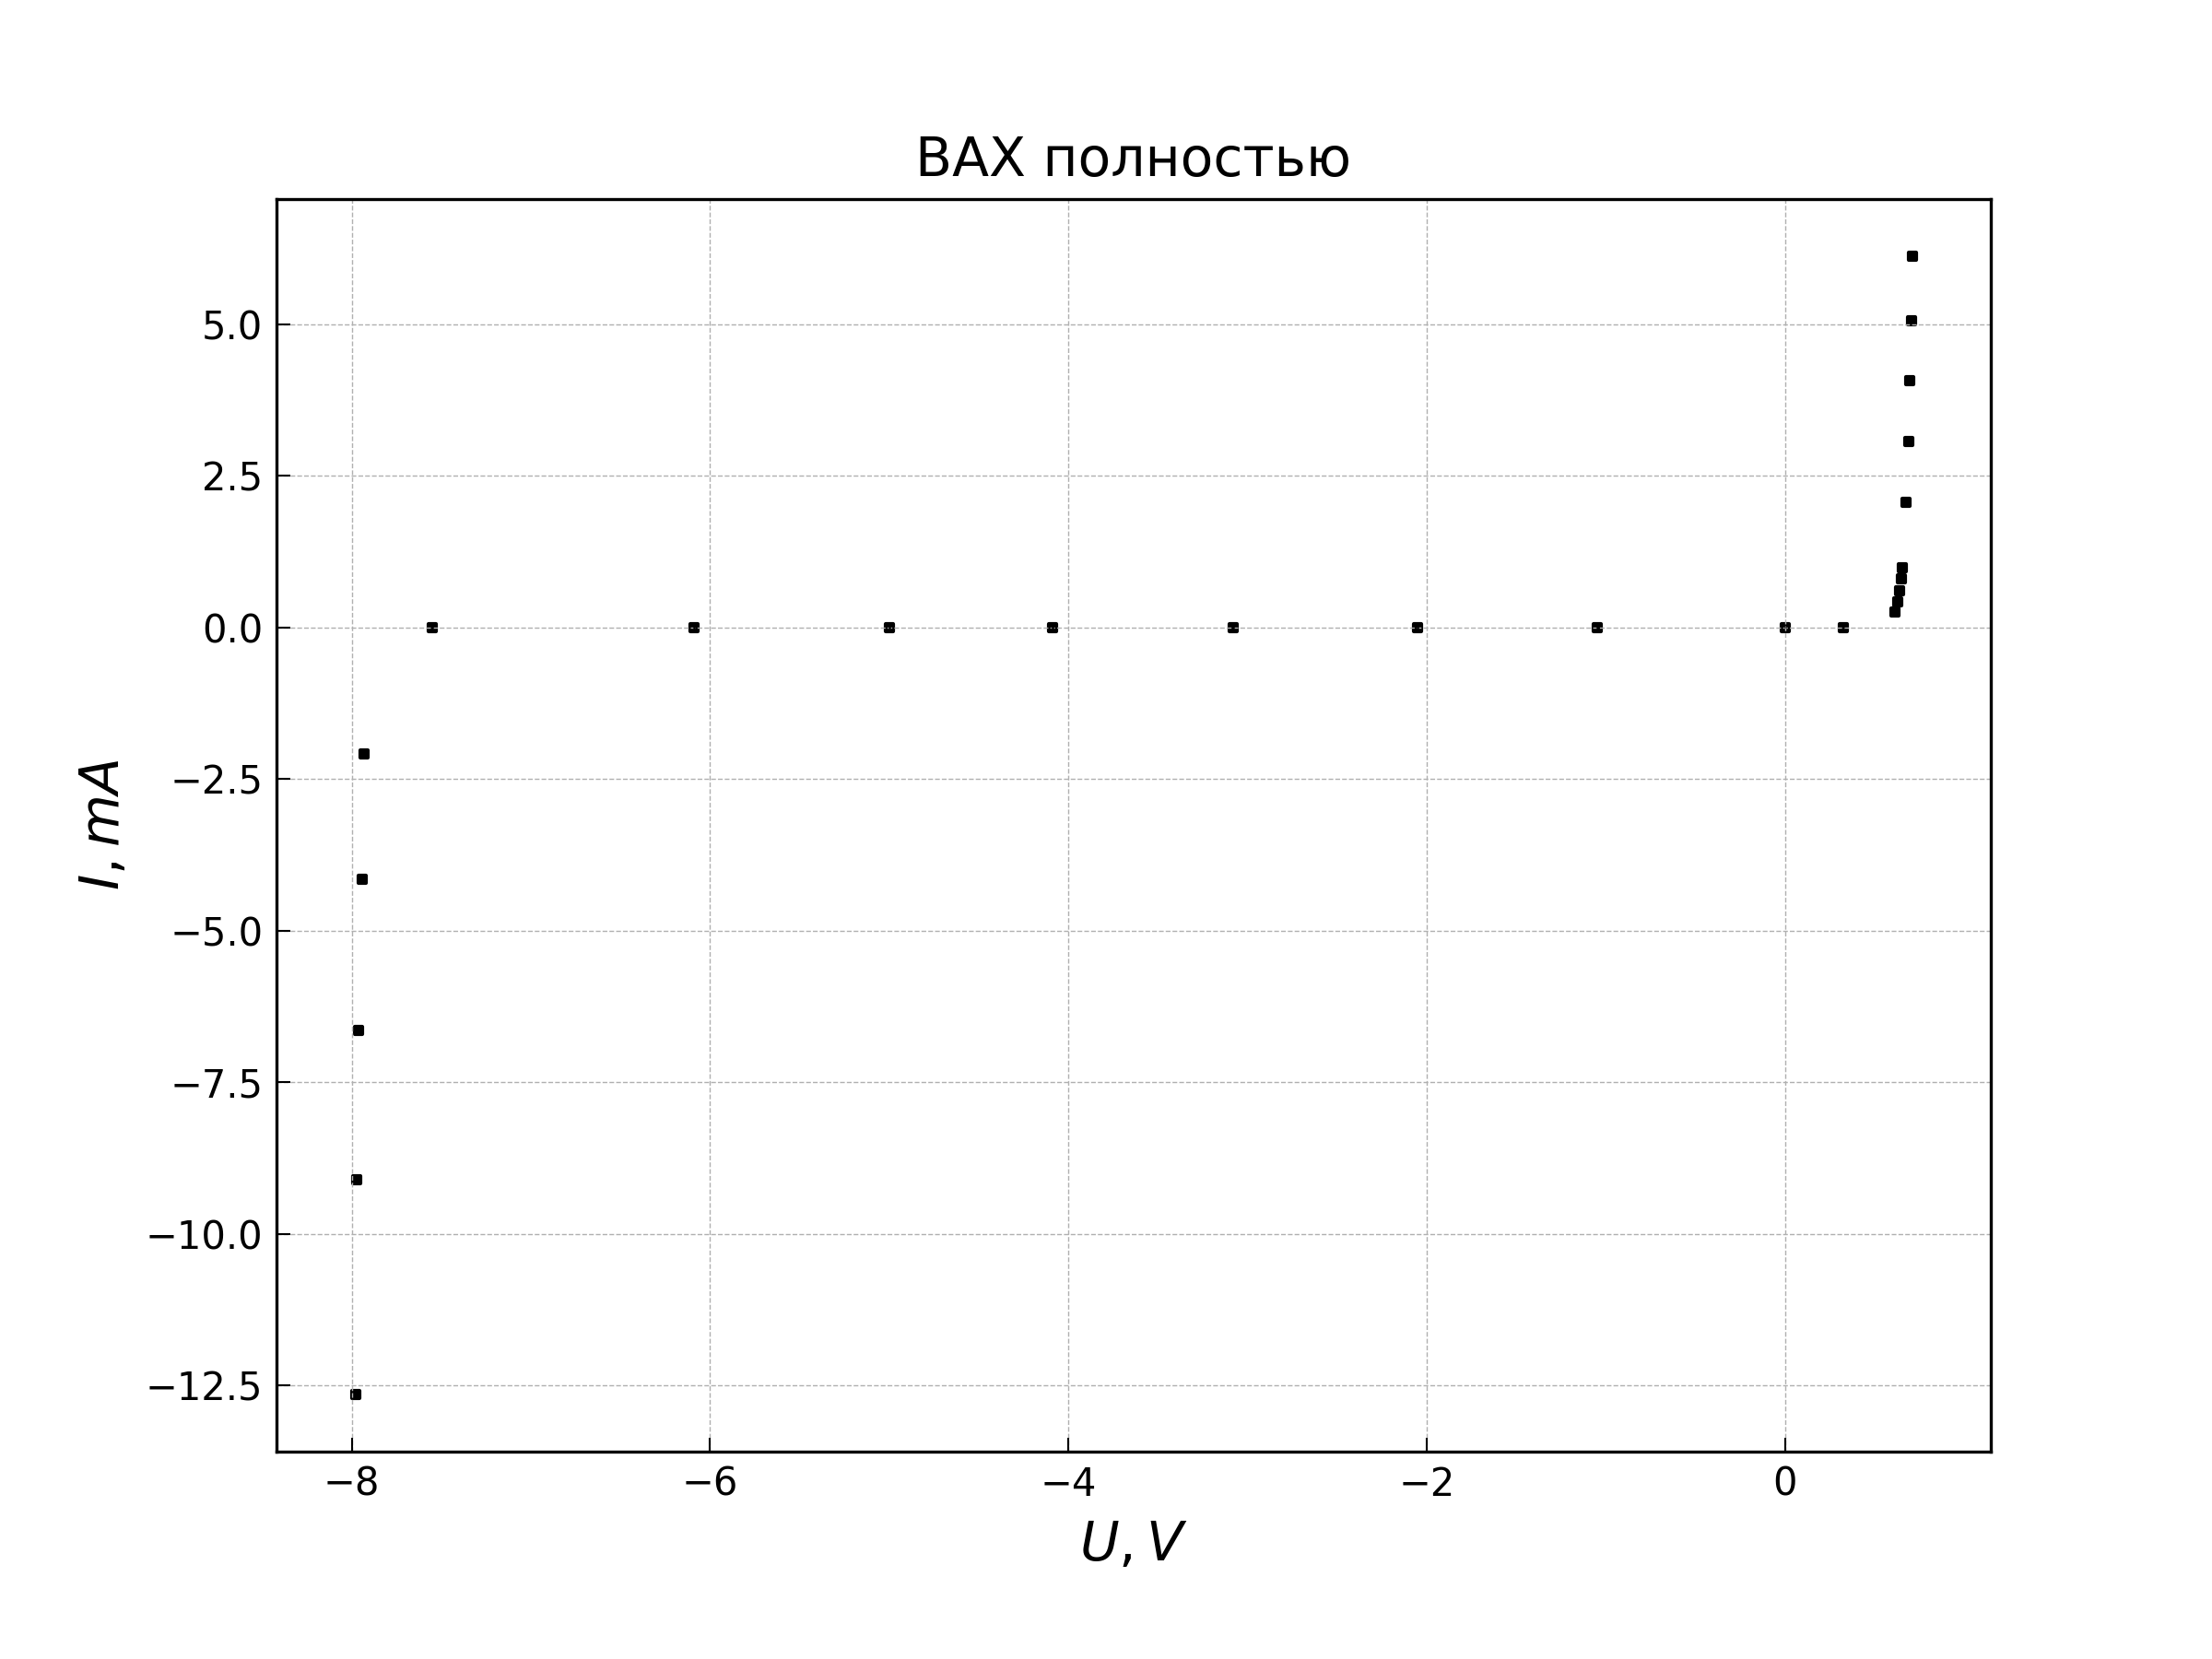
\includegraphics[scale=0.9]{323IUFull.png}}
		\caption{ВАХ диода полностью}
		\label{fig:image}
	\end{figure}
	
	\begin{figure}[H]
		\center{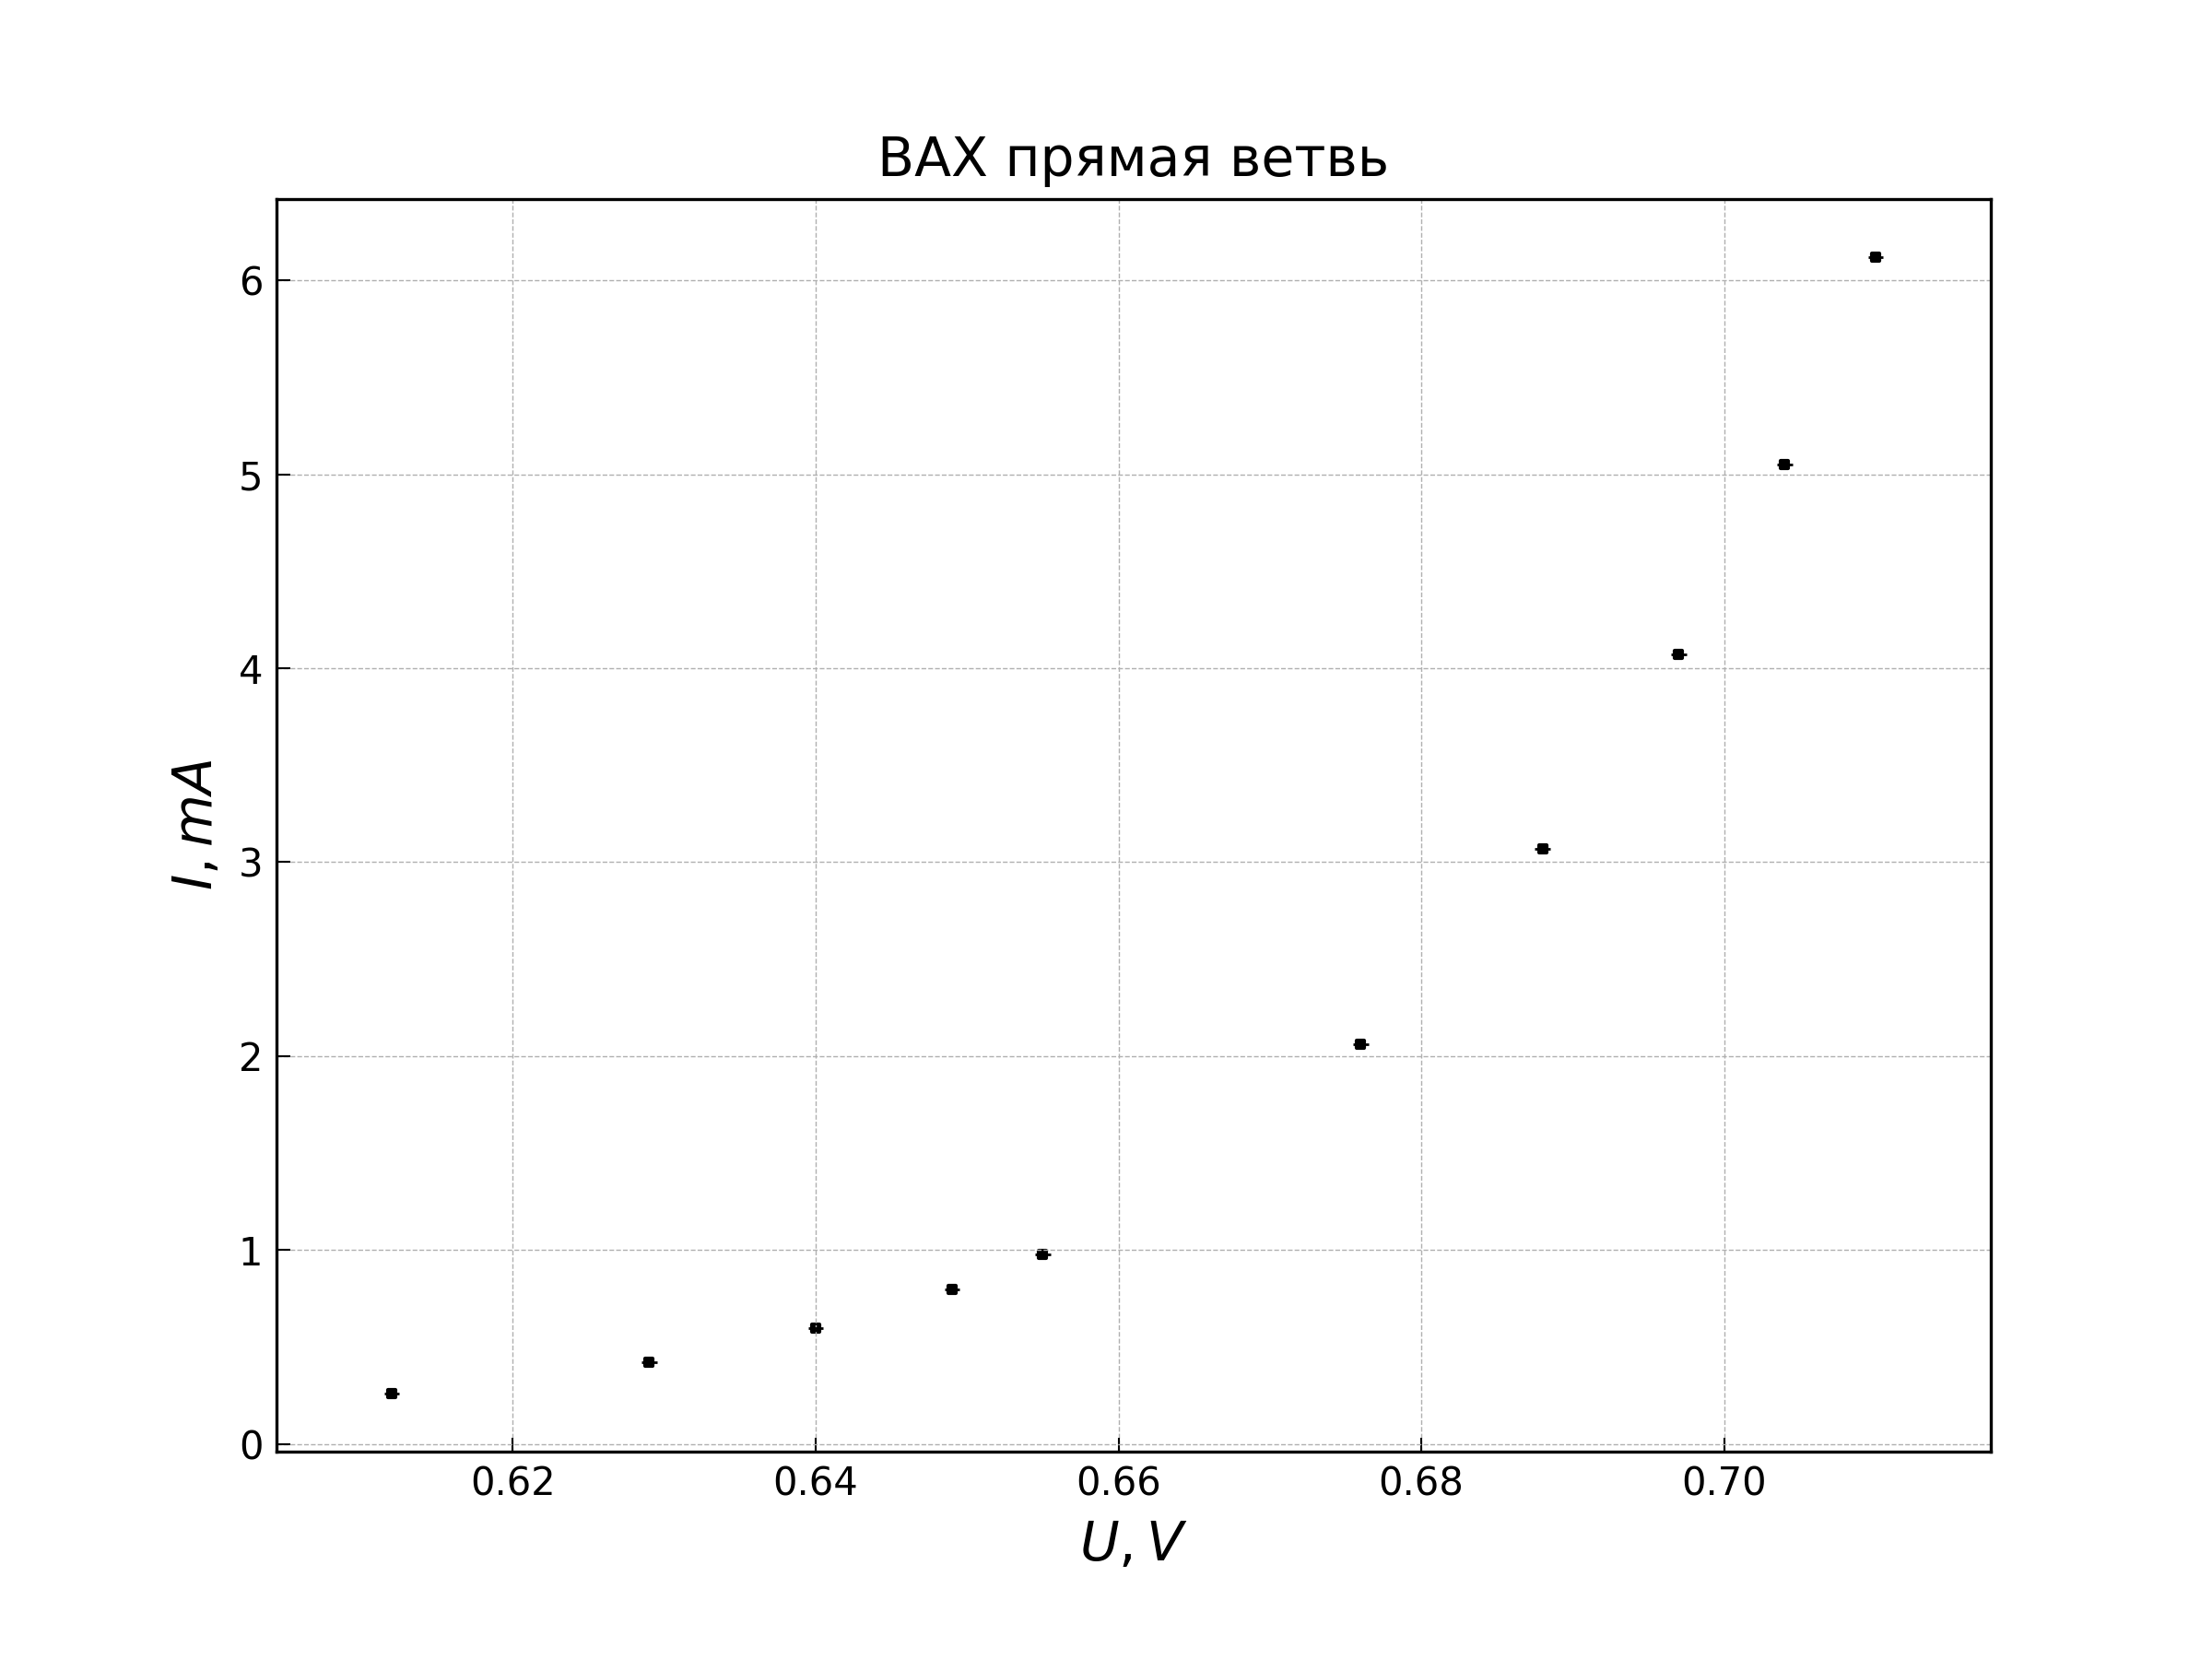
\includegraphics[scale=0.9, angle=90]{323IULine.png}}
		\caption{Прямая ветвь ВАХ}
		\label{fig:image2}
	\end{figure}

\begin{figure}[H]
	\center{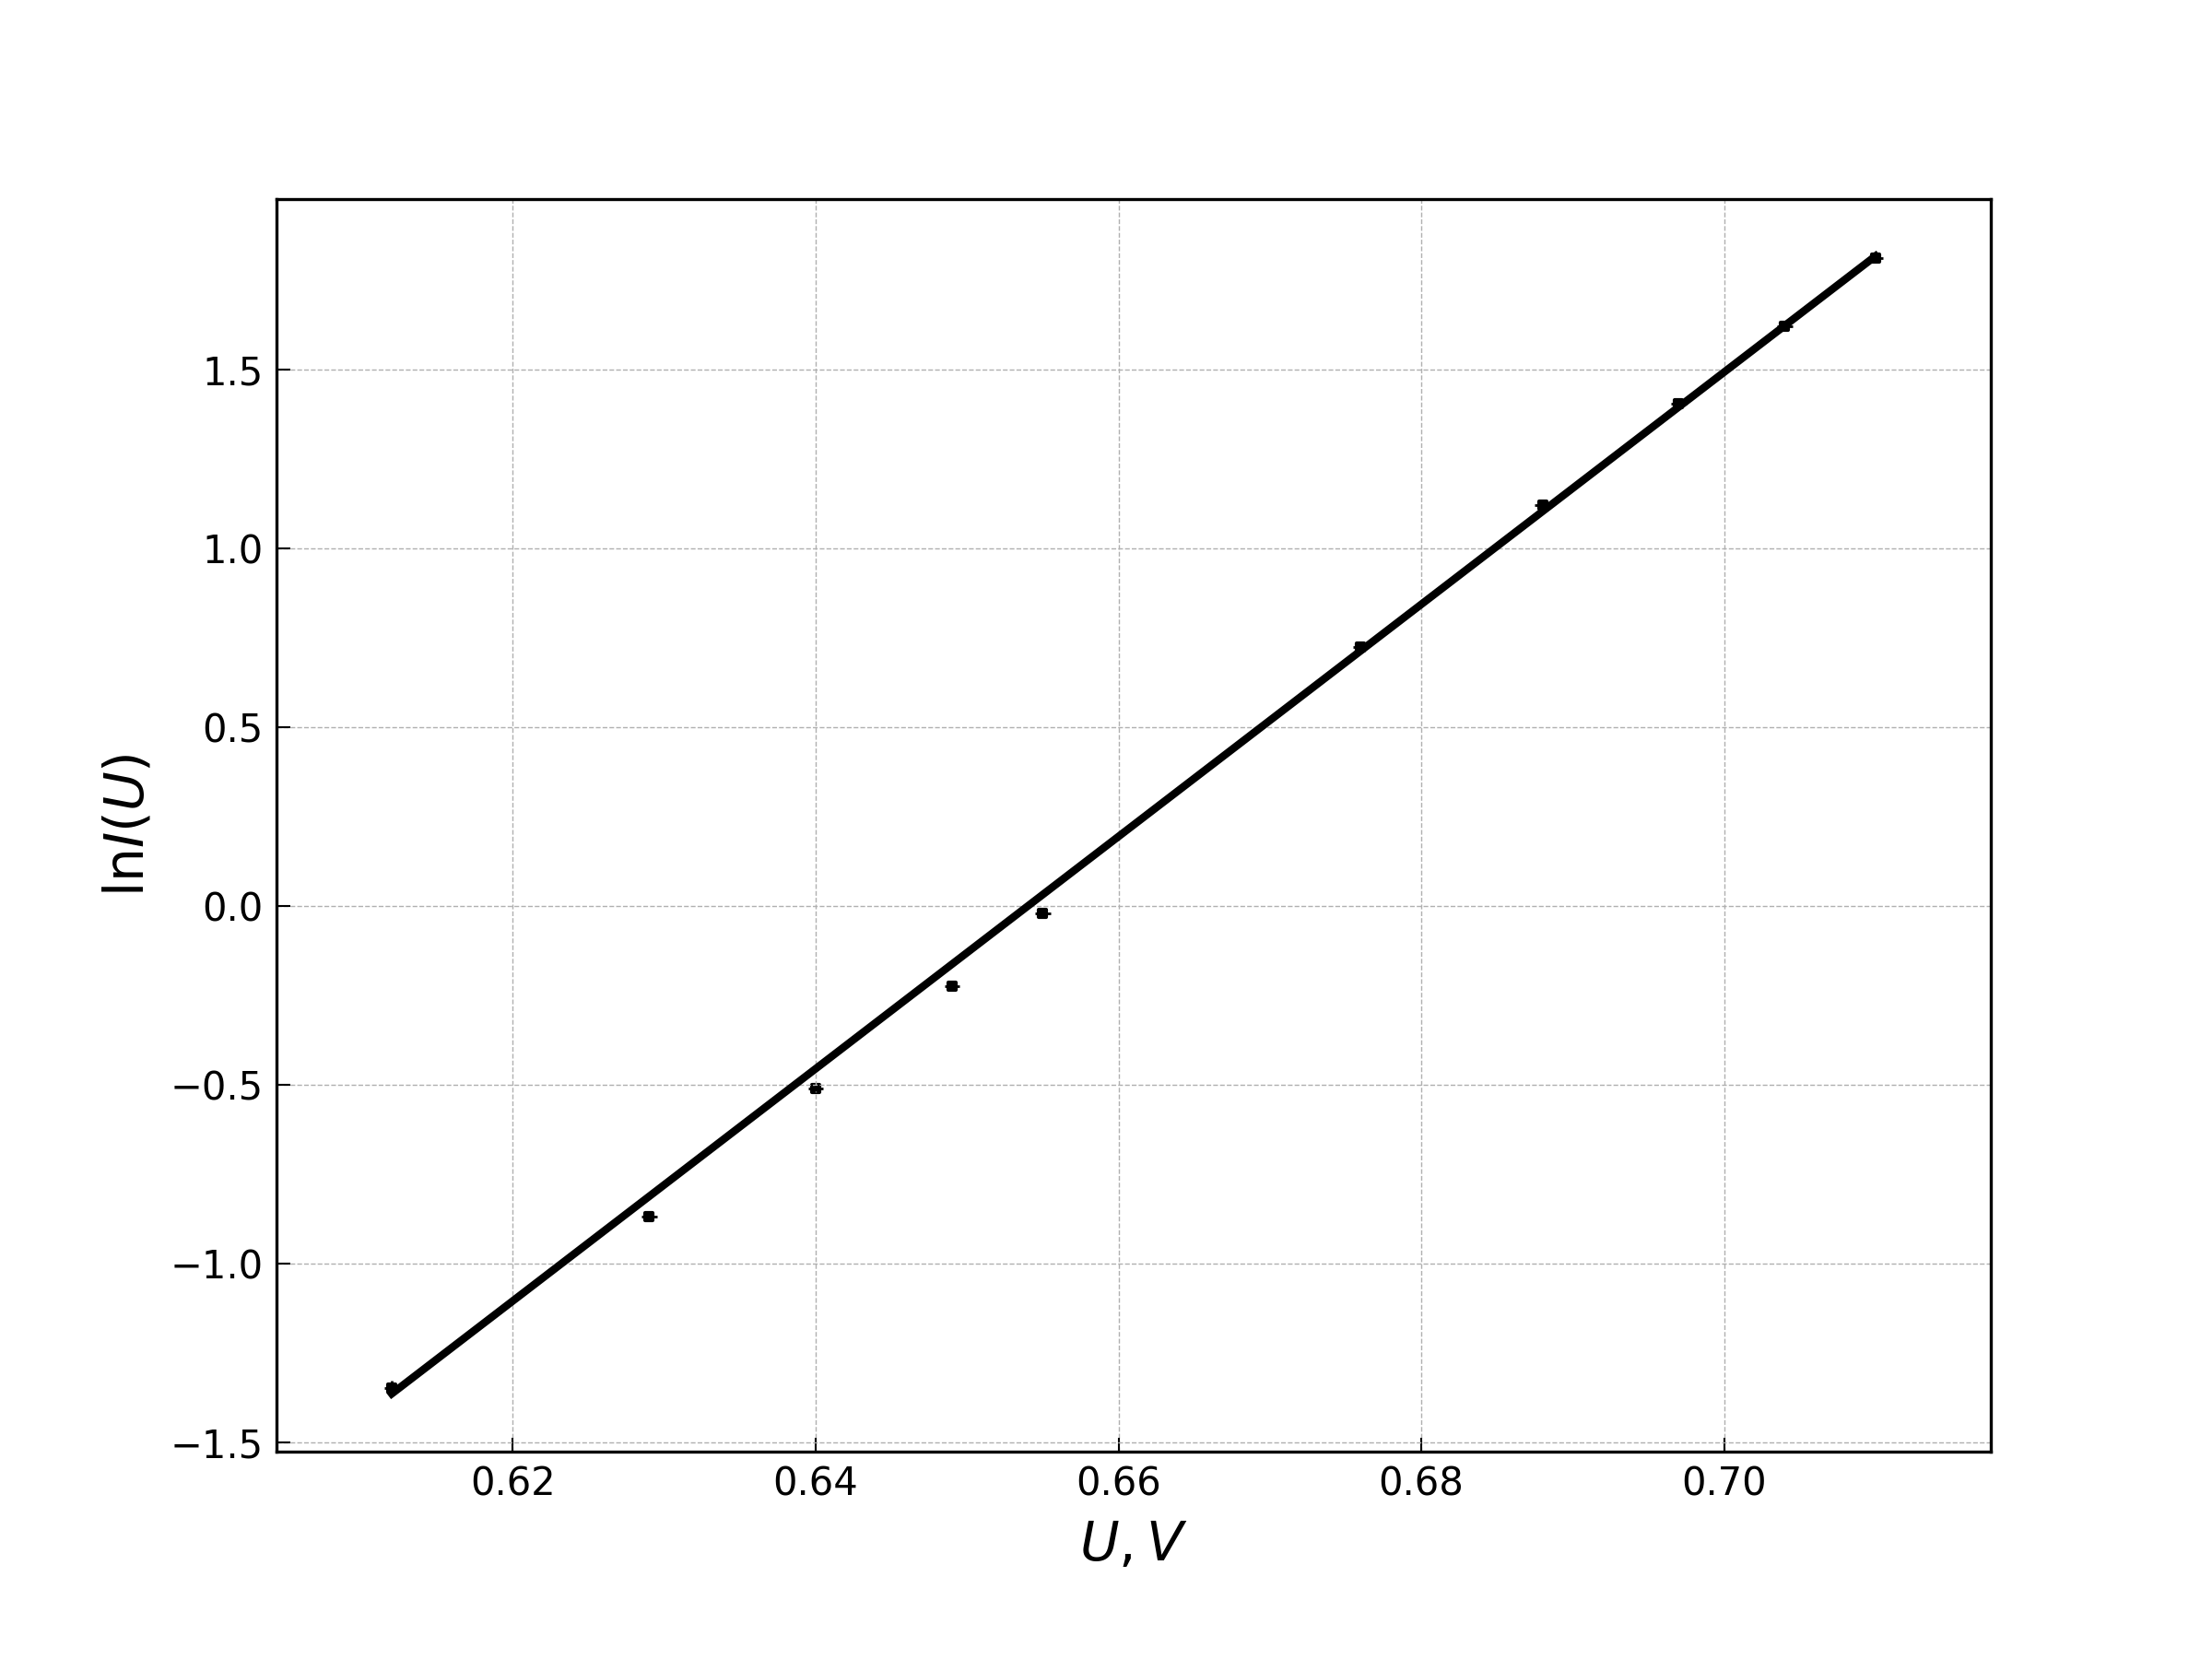
\includegraphics[scale=0.9, angle=90]{323IULineFit.png}}
	\caption{Проверка теоретической зависимости $\ln I(U)$}
	\label{fig:image3}
\end{figure}
	
	
\begin{minipage}{0.4\textwidth}
	\begin{table}[H]
		\begin{tabular}{ll}
			\toprule
			$U,\: V$ &          $I,\: mA$ \\
			\midrule
			0.0000 ± 0.0005 &  0.000 ± 0.005 \\
			0.3260 ± 0.0005 &  0.000 ± 0.005 \\
			0.6120 ± 0.0005 &  0.260 ± 0.005 \\
			0.6290 ± 0.0005 &  0.420 ± 0.005 \\
			0.6400 ± 0.0005 &  0.600 ± 0.005 \\
			0.6490 ± 0.0005 &  0.800 ± 0.005 \\
			0.6550 ± 0.0005 &  0.980 ± 0.005 \\
			0.6760 ± 0.0005 &  2.060 ± 0.005 \\
			0.6880 ± 0.0005 &  3.070 ± 0.005 \\
			0.6970 ± 0.0005 &  4.070 ± 0.005 \\
			0.7040 ± 0.0005 &  5.050 ± 0.005 \\
			0.7100 ± 0.0005 &  6.120 ± 0.005 \\
			\bottomrule
		\end{tabular}
	\caption{Вольтамперная характеристика диода (прямая ветвь) }
	\end{table}
\end{minipage}
\hfill
\begin{minipage}{0.4\textwidth}
	\begin{table}[H]
		\begin{tabular}{ll}
			\toprule
			$U,\: V$ &          $I,\: mA$ \\
			\midrule
			-1.050 ± 0.005 &    0.000 ± 0.005 \\
			-2.050 ± 0.005 &    0.000 ± 0.005 \\
			-3.080 ± 0.005 &    0.000 ± 0.005 \\
			-4.090 ± 0.005 &    0.000 ± 0.005 \\
			-5.000 ± 0.005 &    0.000 ± 0.005 \\
			-6.090 ± 0.005 &    0.000 ± 0.005 \\
			-7.550 ± 0.005 &    0.000 ± 0.005 \\
			-7.930 ± 0.005 &   -2.080 ± 0.005 \\
			-7.940 ± 0.005 &   -4.150 ± 0.005 \\
			-7.960 ± 0.005 &   -6.650 ± 0.005 \\
			-7.970 ± 0.005 &   -9.110 ± 0.005 \\
			-7.980 ± 0.005 &  -12.650 ± 0.005 \\
			\bottomrule
		\end{tabular}
	\caption{Вольтамперная характеристика диода (обратная ветвь)}
	\end{table}
	
\end{minipage}

$\ln I(U) = A \: U + B \Longrightarrow \left\lbrace \begin{array}{c}
A = 32.5 \pm 0.3 \: V^{-1}\\ 
B = -21.2 \pm 0.2\\ 
r \approx 0.9996
\end{array}\right. $

\section*{Упражнение 2}
\indent
  
  \begin{table}[H]
  \begin{tabular}{ll}
  	\toprule
  	$U,\: V$ &          $C,\: nF$ \\
  	\midrule
  	-0.030 ± 0.005 &  0.280 ± 0.005 \\
  	-0.510 ± 0.005 &  0.160 ± 0.005 \\
  	-1.040 ± 0.005 &  0.100 ± 0.005 \\
  	-1.510 ± 0.005 &  0.060 ± 0.005 \\
  	0.100 ± 0.005 &  0.380 ± 0.005 \\
  	0.150 ± 0.005 &  0.440 ± 0.005 \\
  	\bottomrule
  \end{tabular}
\caption{Зависимость барьерной ёмкости диода от напряжения}
\end{table}

\begin{figure}[H]
	\center{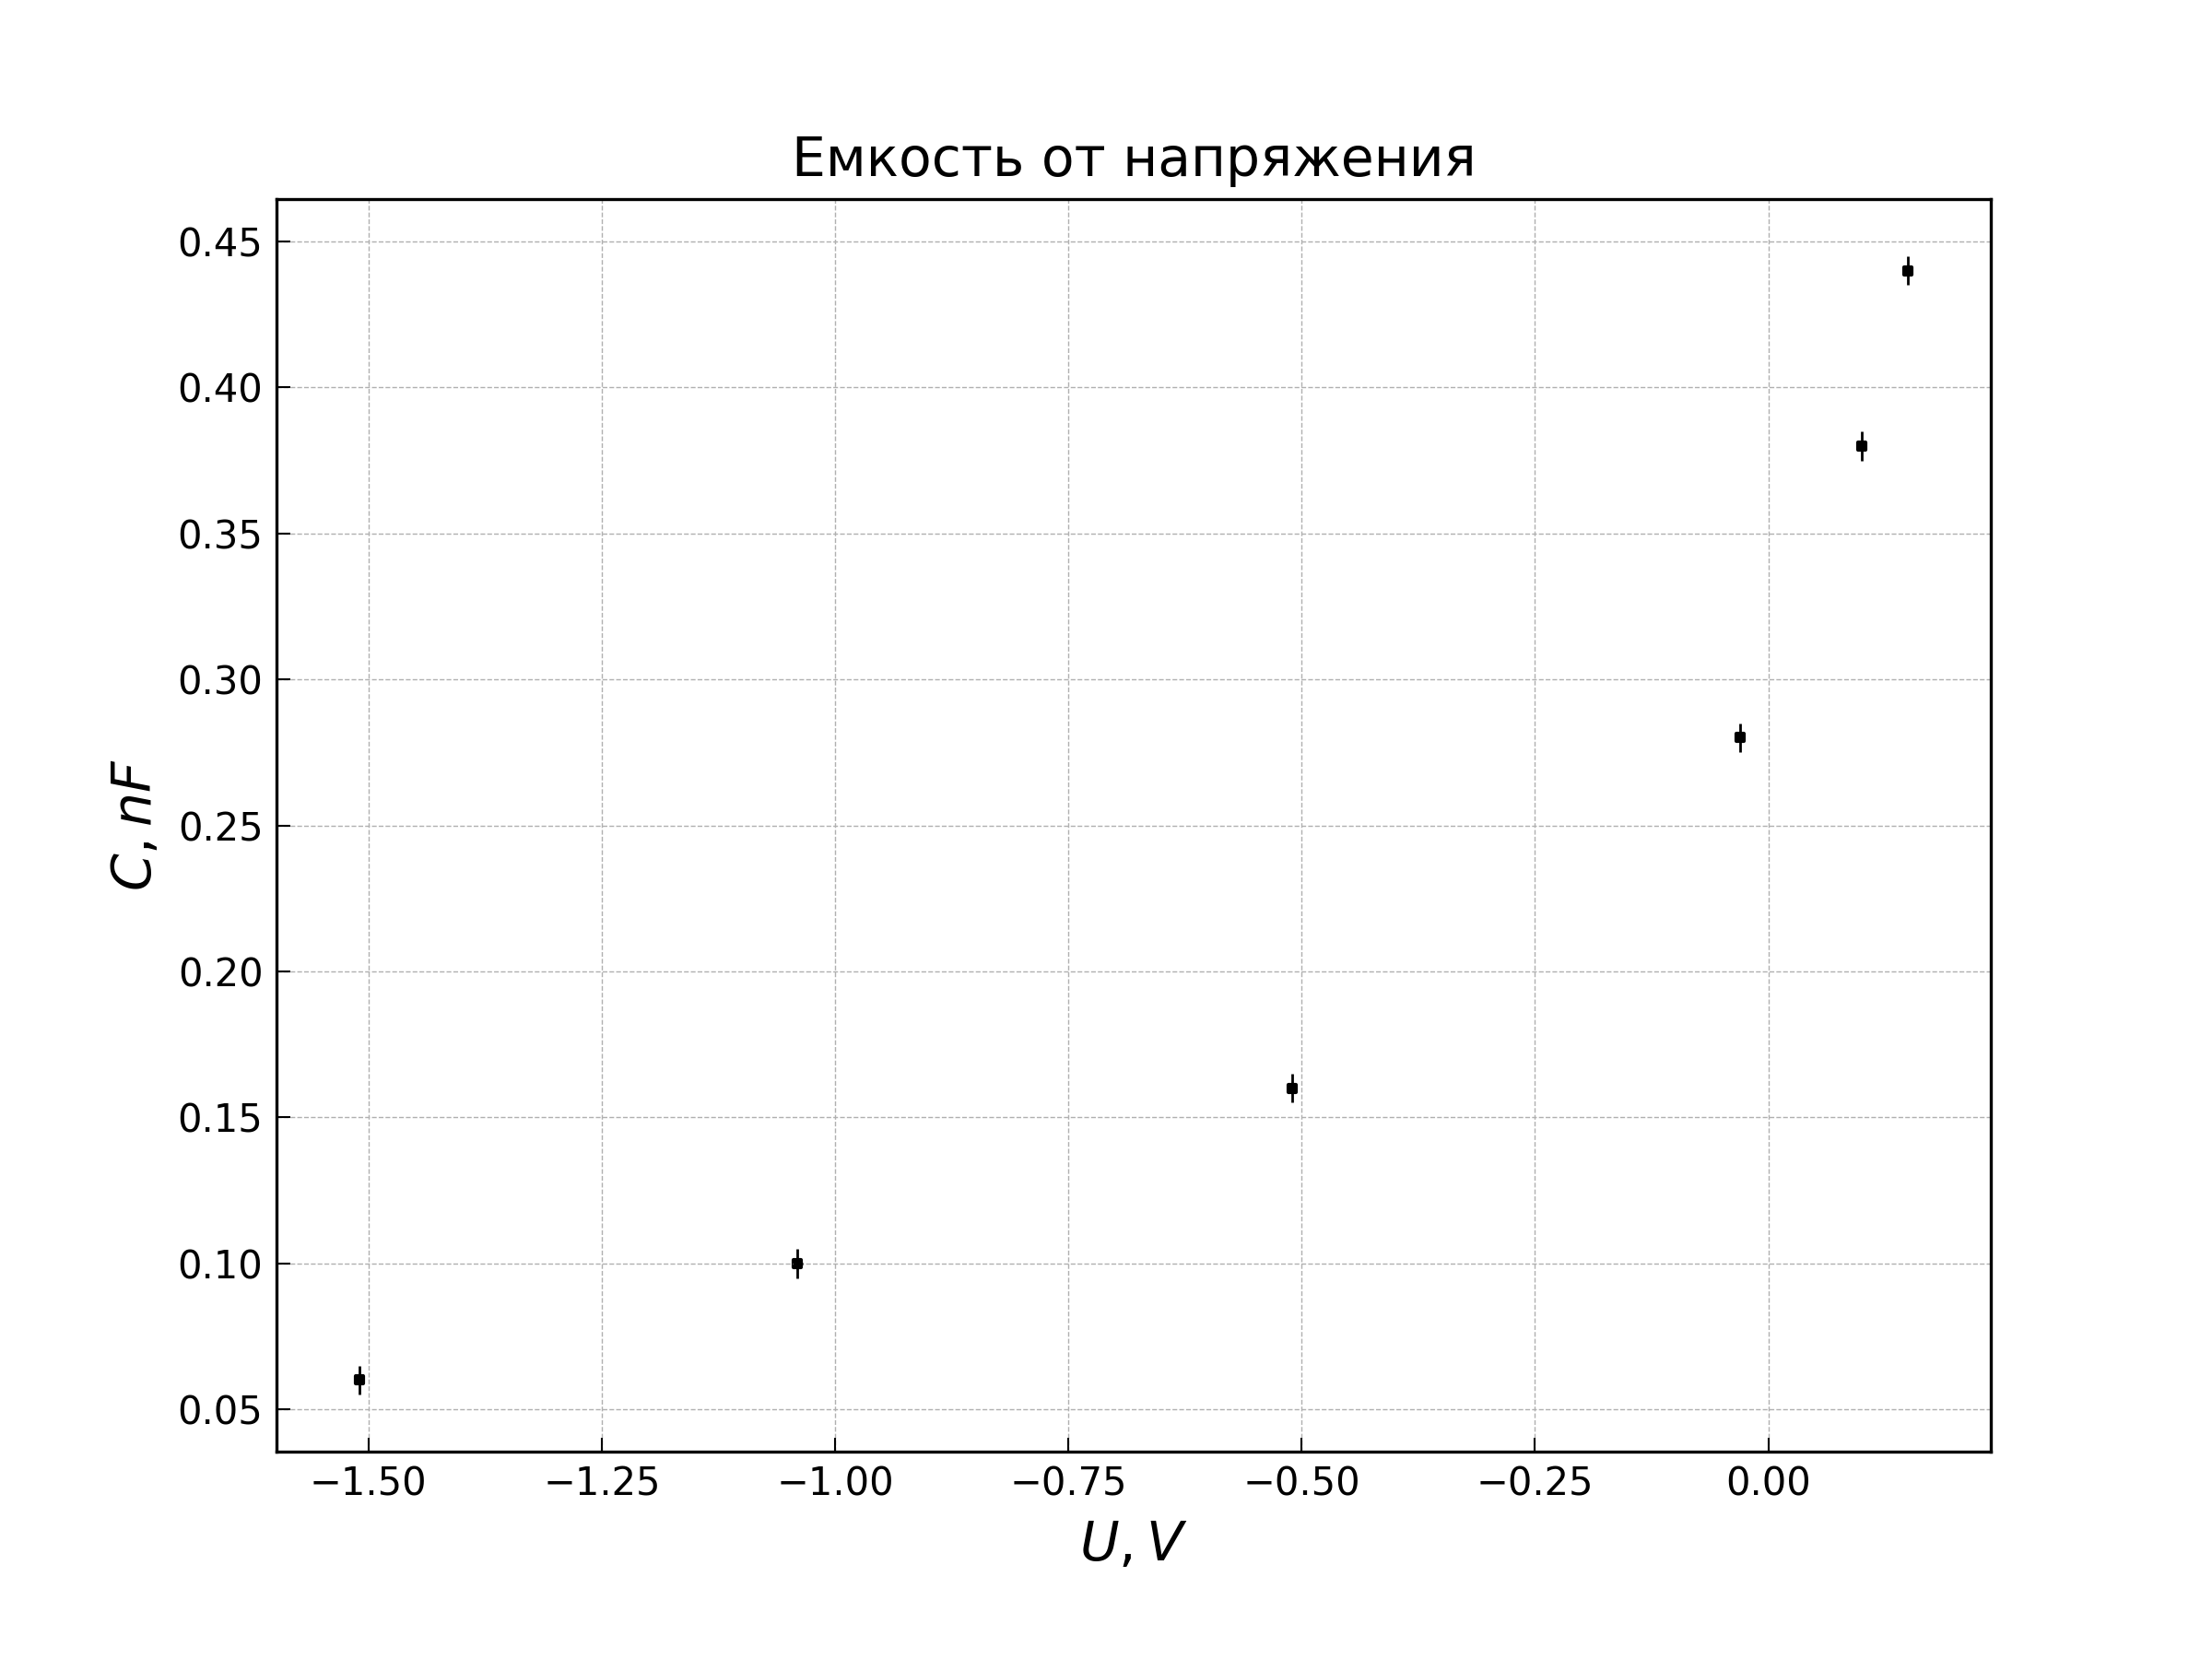
\includegraphics[scale=0.90, angle=90]{323CU.png}}
	\caption{Зависимость барьерной ёмкости диода от напряжения}
	\label{fig:image4}
\end{figure}

\section*{Упражнение 3}
  
  \begin{table}[H]
  \begin{tabular}{ll}
  	\toprule
  	$t,\: ^{\circ}C$ &             $U,\: V$ \\
  	\midrule
  	23.0 ± 0.5 &  0.7040 ± 0.0005 \\
  	40.0 ± 0.5 &  0.6700 ± 0.0005 \\
  	60.0 ± 0.5 &  0.6400 ± 0.0005 \\
  	80.0 ± 0.5 &  0.6000 ± 0.0005 \\
  	\bottomrule
  \end{tabular}
\caption{Зависимость напряжения на диоде от температуры}
\end{table}

\begin{figure}[H]
	\center{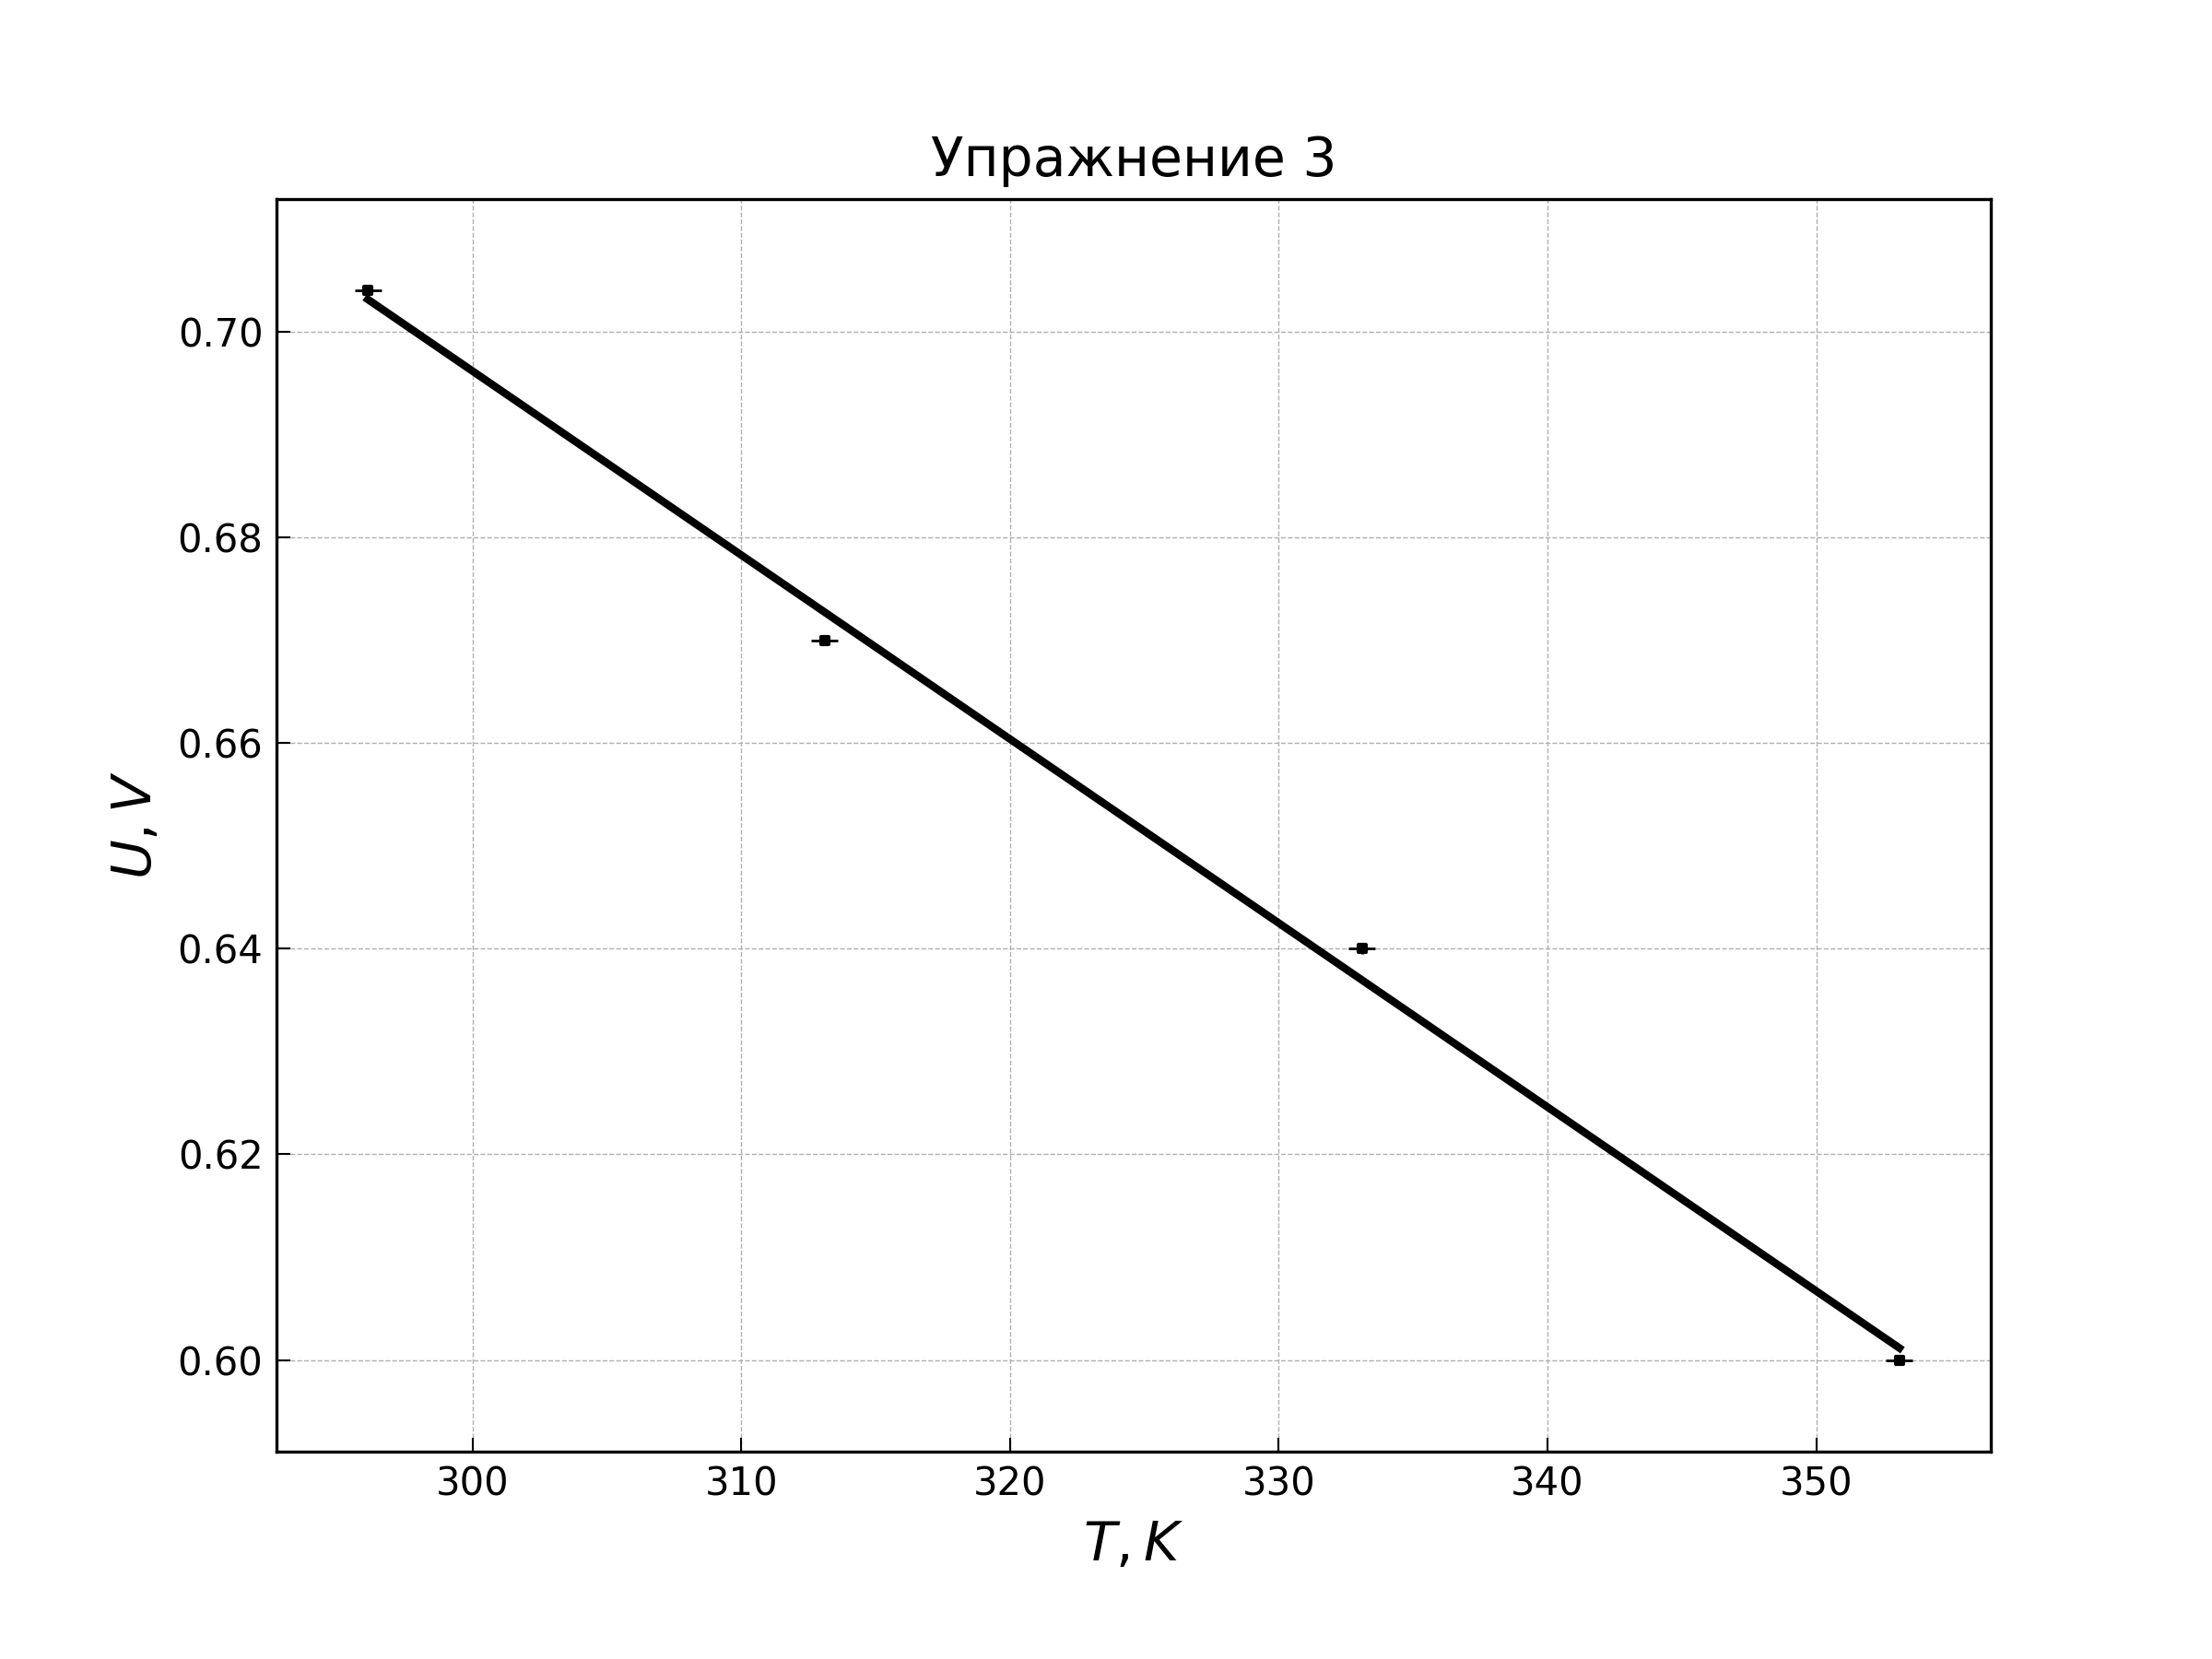
\includegraphics[scale=0.7, angle=0]{323TU.png}}
	\caption{Зависимость напряжения на диоде от температуры}
	\label{fig:image5}
\end{figure}

$U = A \: T + B \Longrightarrow \left\lbrace \begin{array}{c}
A = -0.00179 \pm 0.00007 \: V \cdot K^{-1}\\ 
B = 1.23 \pm 0.02 \: V\\ 
r \approx -0.9984
\end{array}\right. $


\section*{Упражнение 4}

\begin{figure}[H]
	\begin{minipage}[h]{0.47\linewidth}
		\center{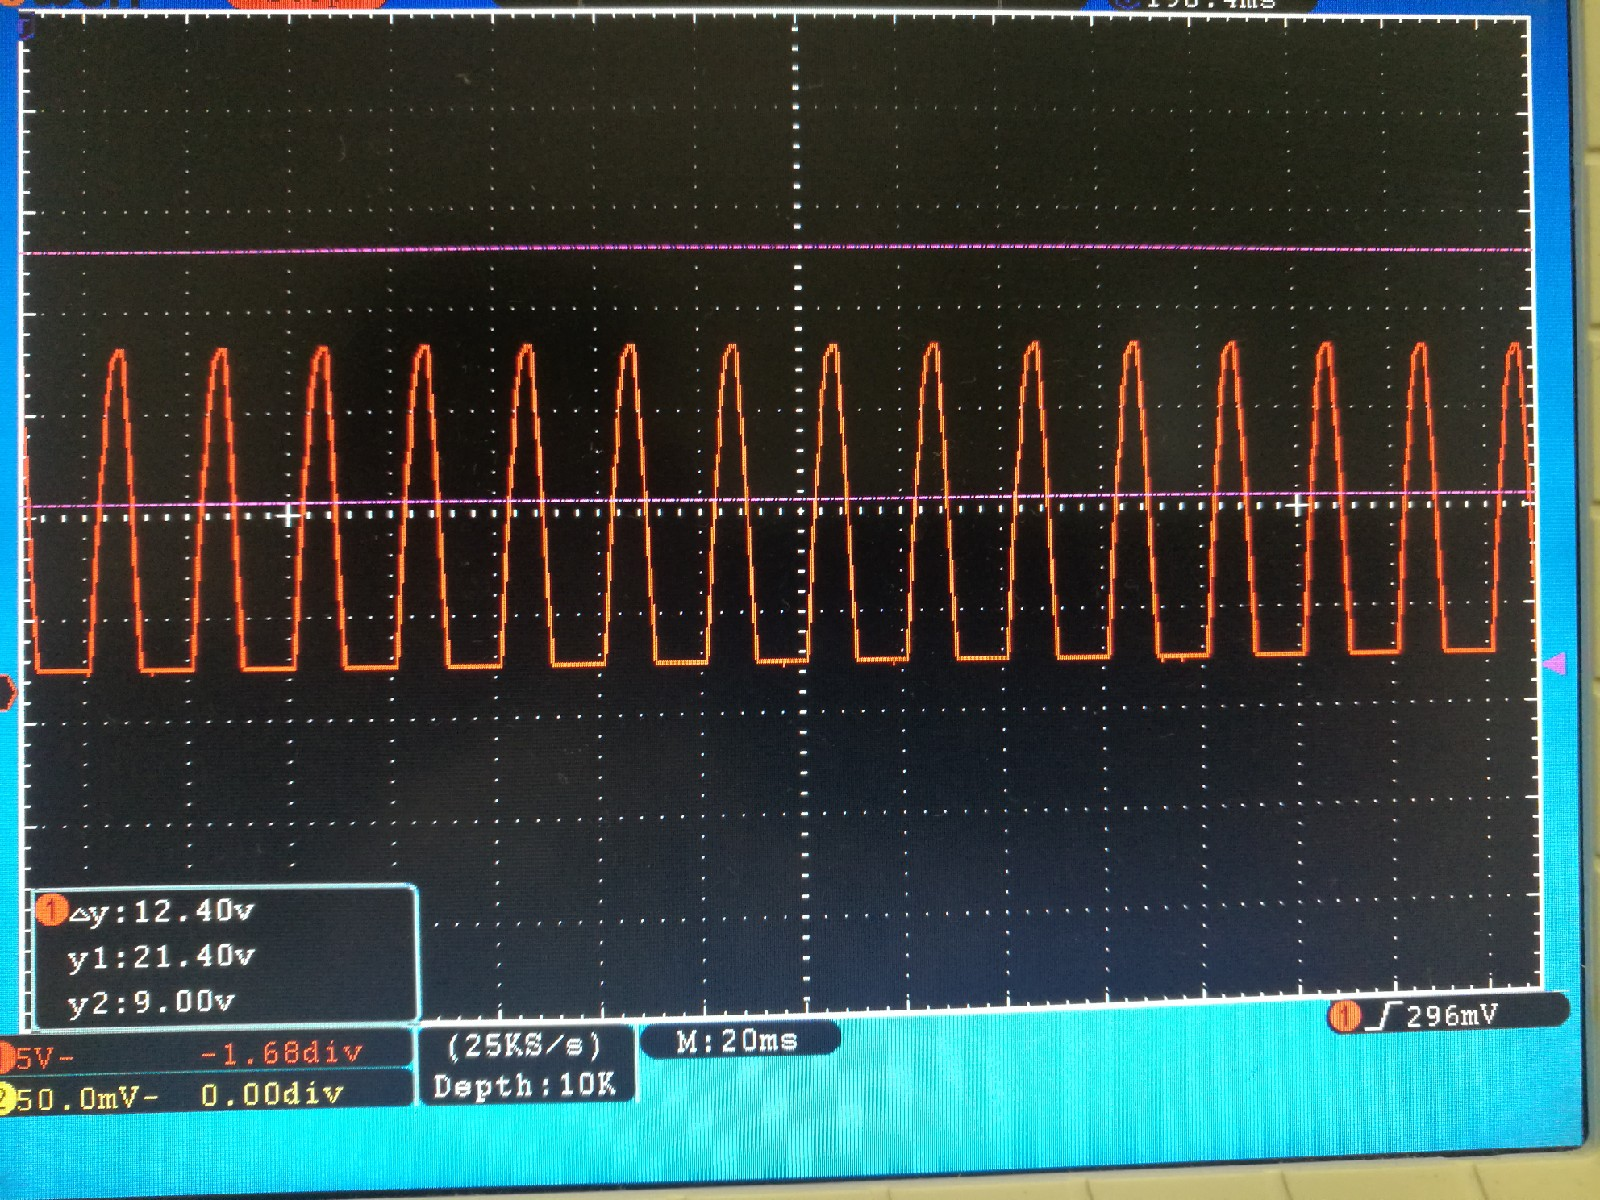
\includegraphics[width=1\linewidth]{1.jpg}} a) \\
	\end{minipage}
	\hfill
	\begin{minipage}[h]{0.47\linewidth}
		\center{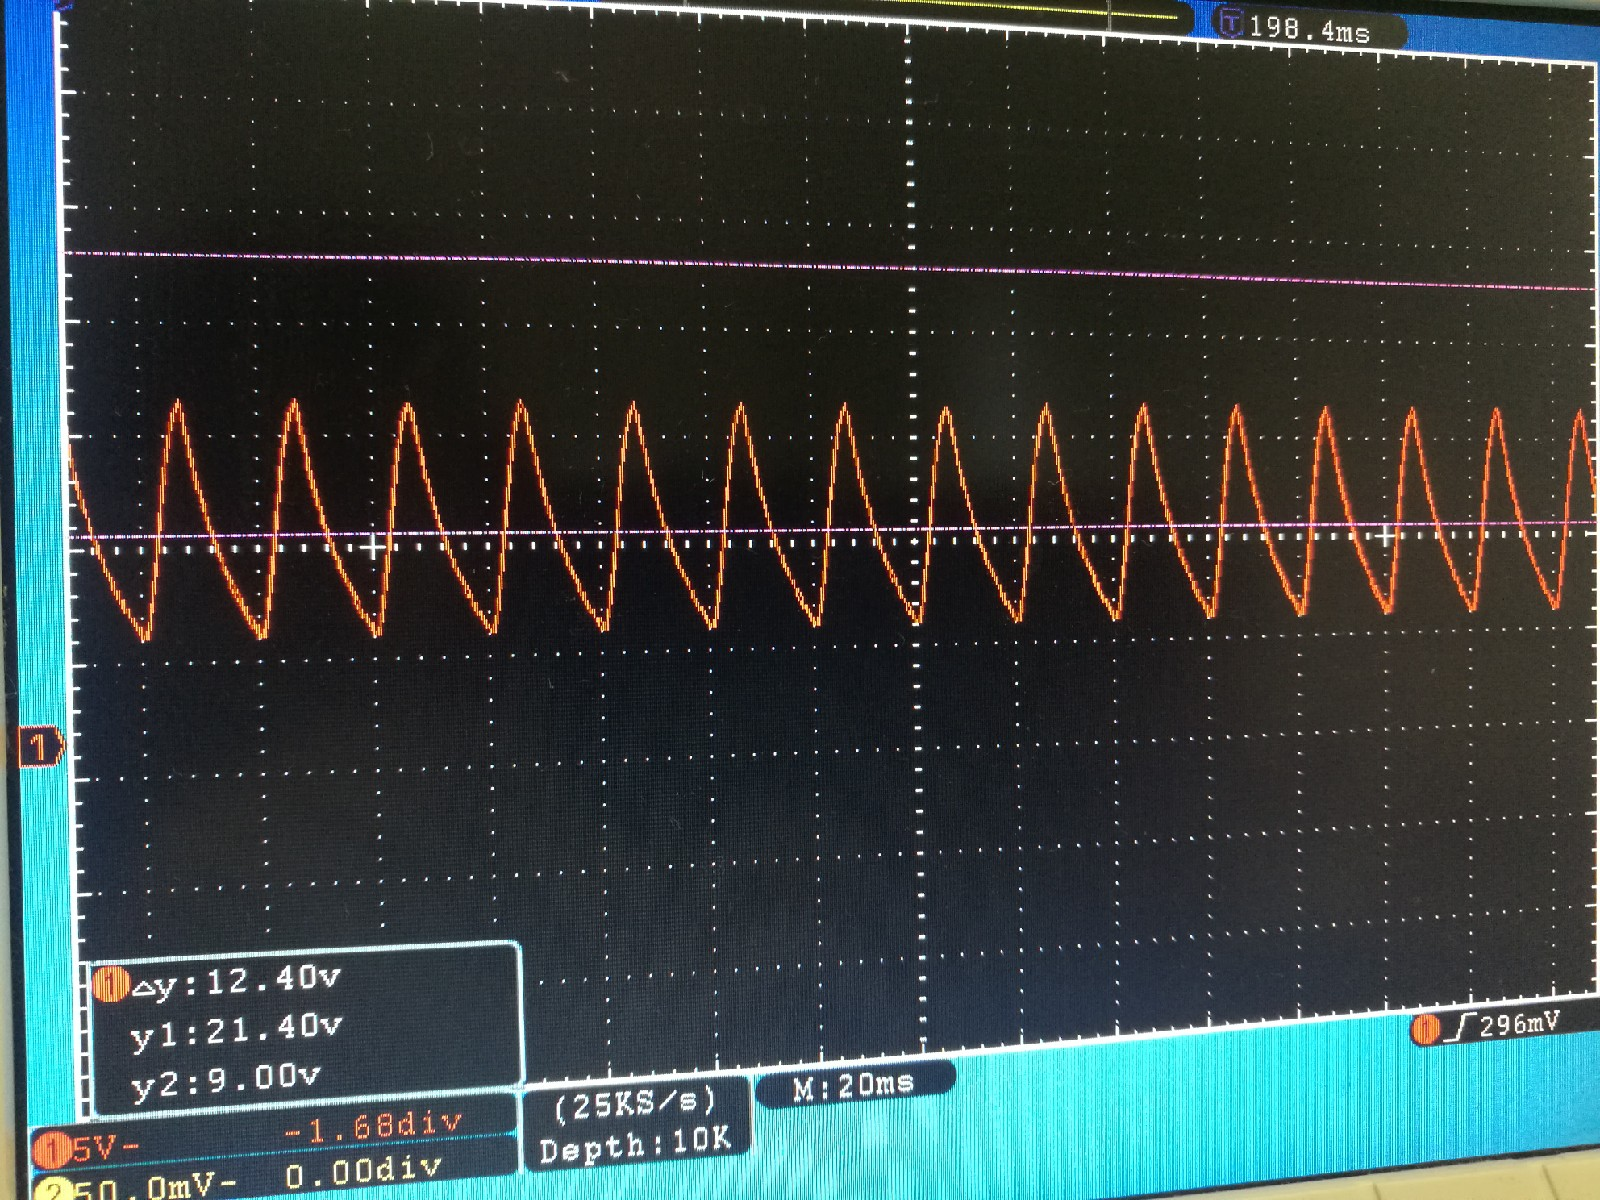
\includegraphics[width=1\linewidth]{2.jpg}} \\b)
	\end{minipage}
	\vfill
	\begin{minipage}[h]{0.47\linewidth}
		\center{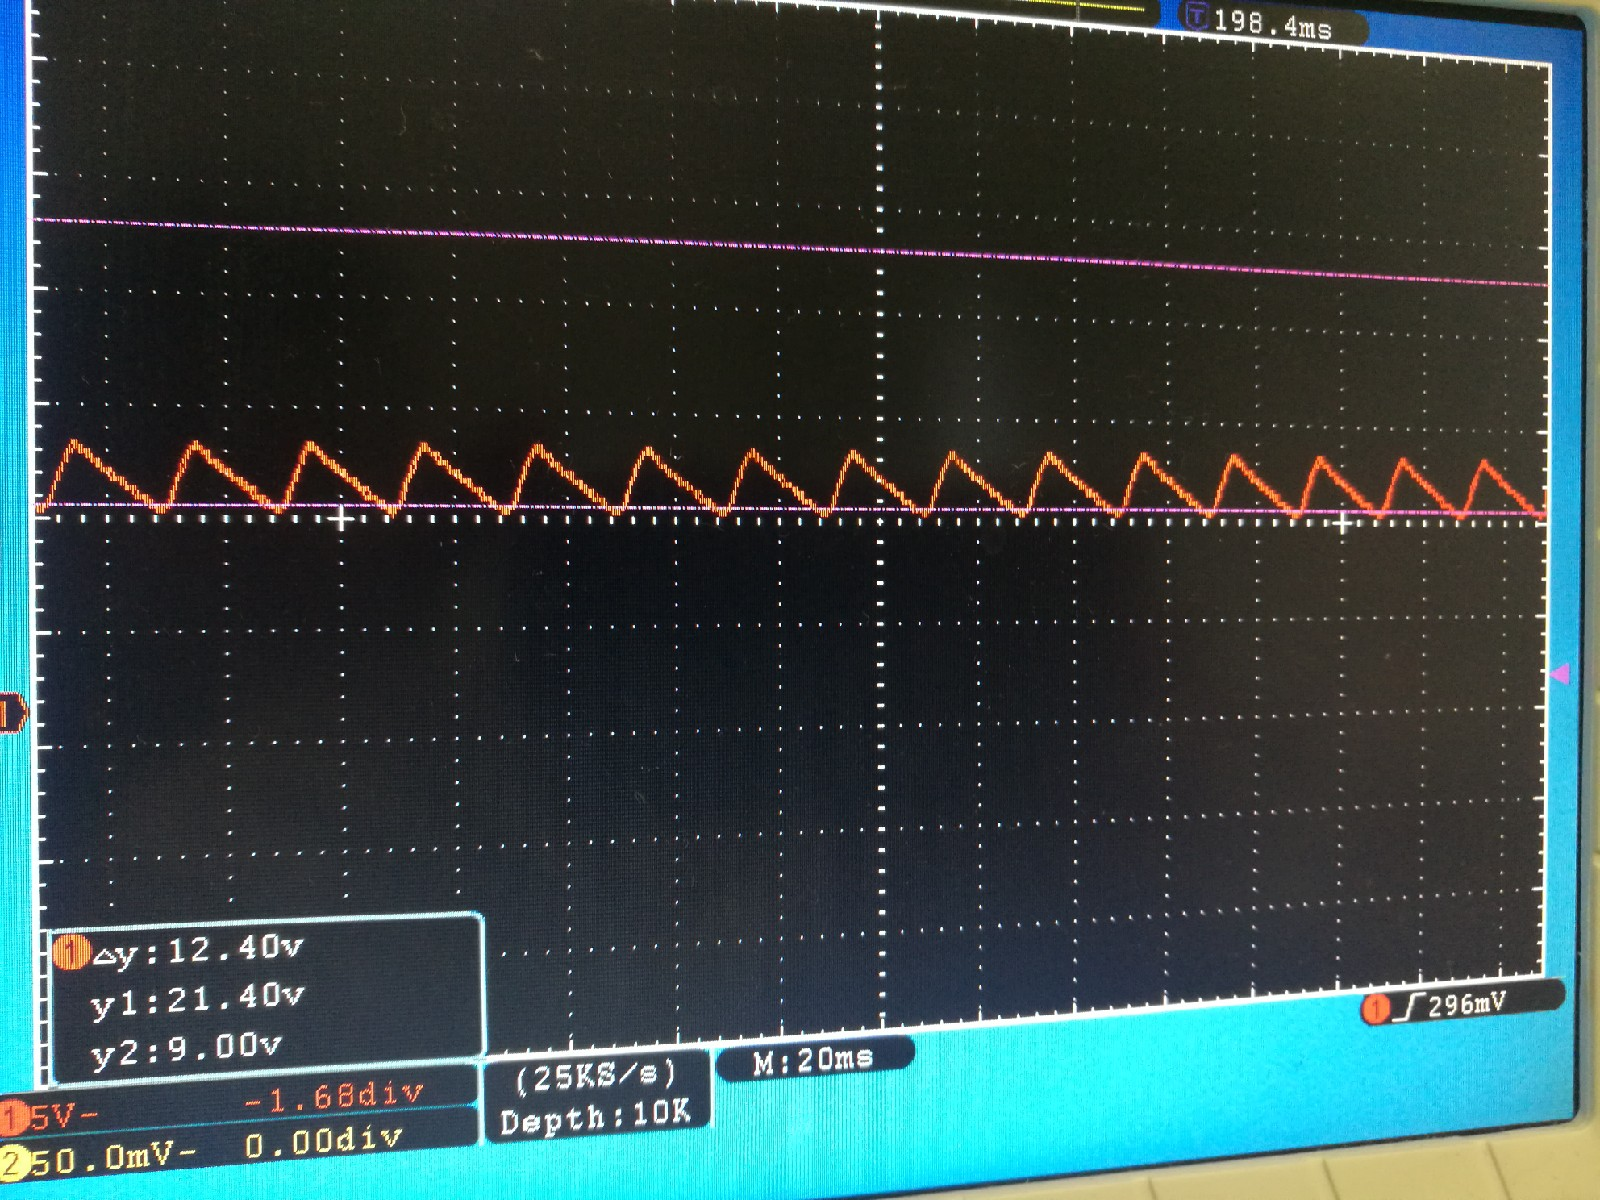
\includegraphics[width=1\linewidth]{3.jpg}} c) \\
	\end{minipage}
	\hfill
	\begin{minipage}[h]{0.47\linewidth}
		\center{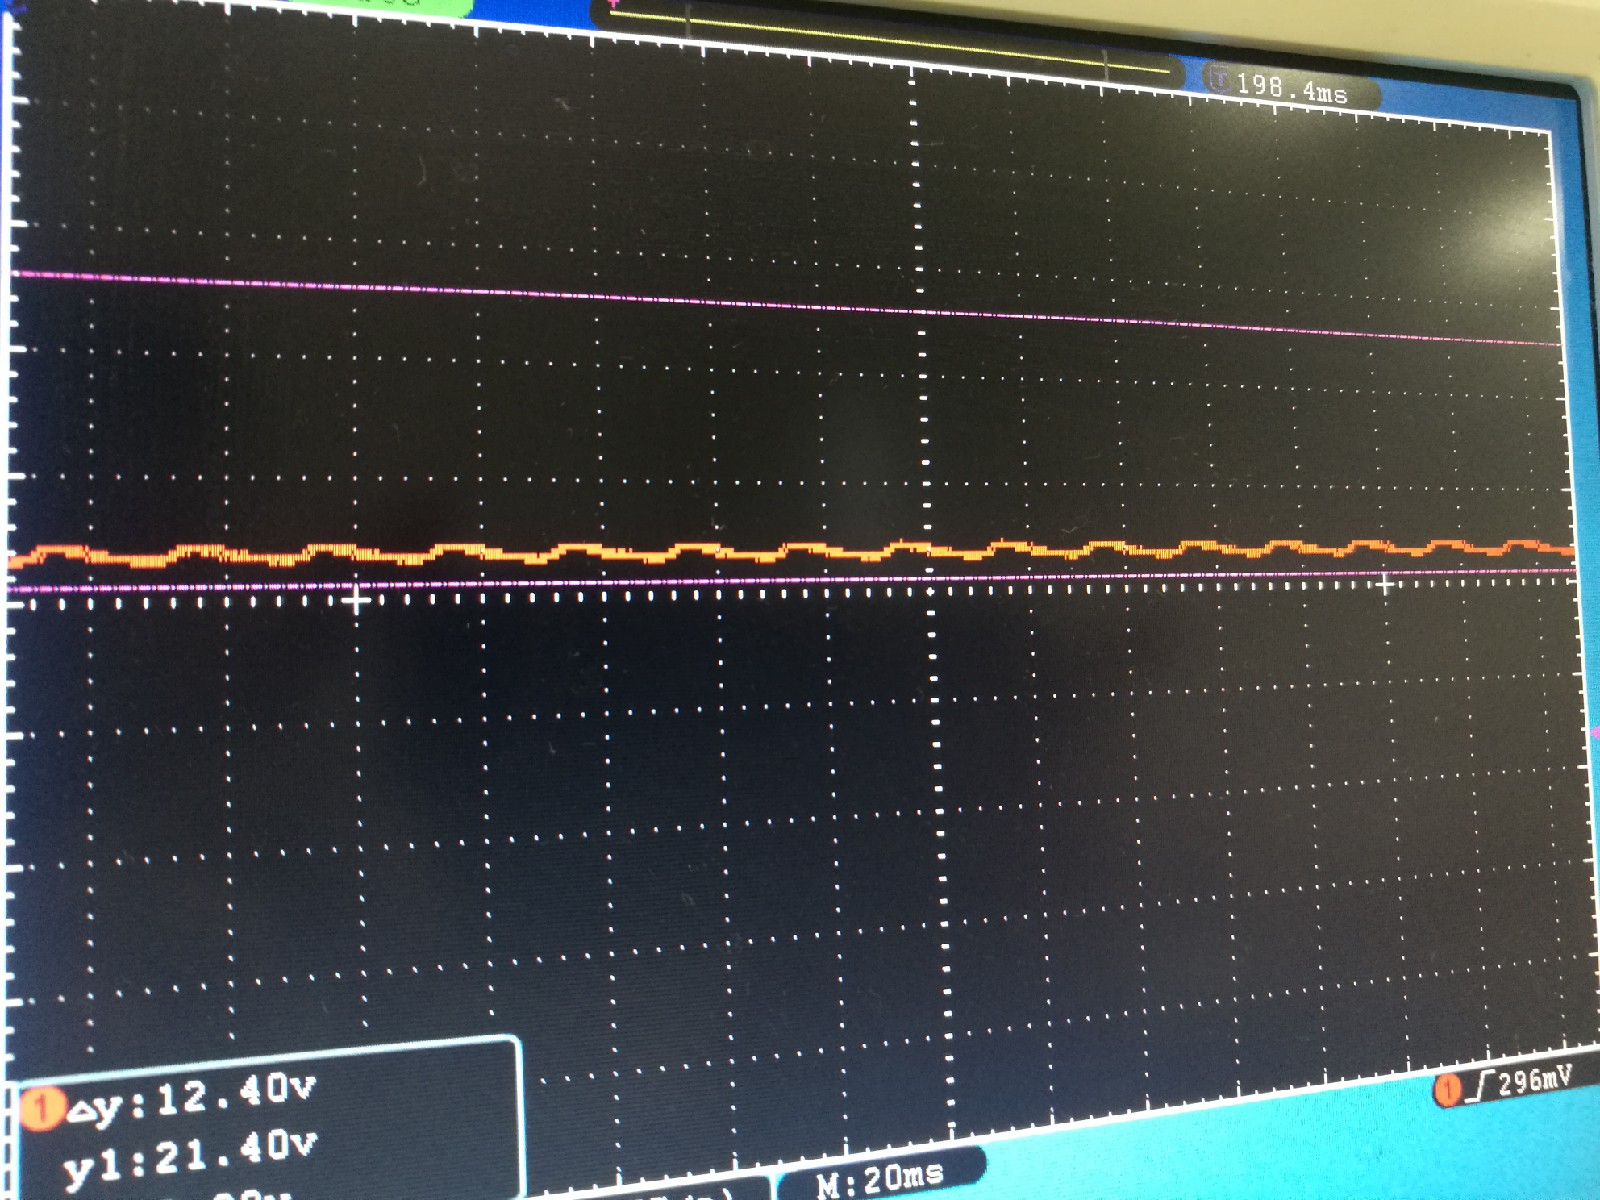
\includegraphics[width=1\linewidth]{4.jpg}} d) \\
	\end{minipage}
	\caption{Осциллограммы напряжения на выходе однополупериодного выпрямителя со сглаживающими емкостями a)$C = 0$; b)$C_1$; c)$C_2 > C_1$; d)$C_3 > C_2$.}
	\label{ris:image6}
\end{figure}

\begin{figure}[H]
	\begin{minipage}[h]{0.47\linewidth}
		\center{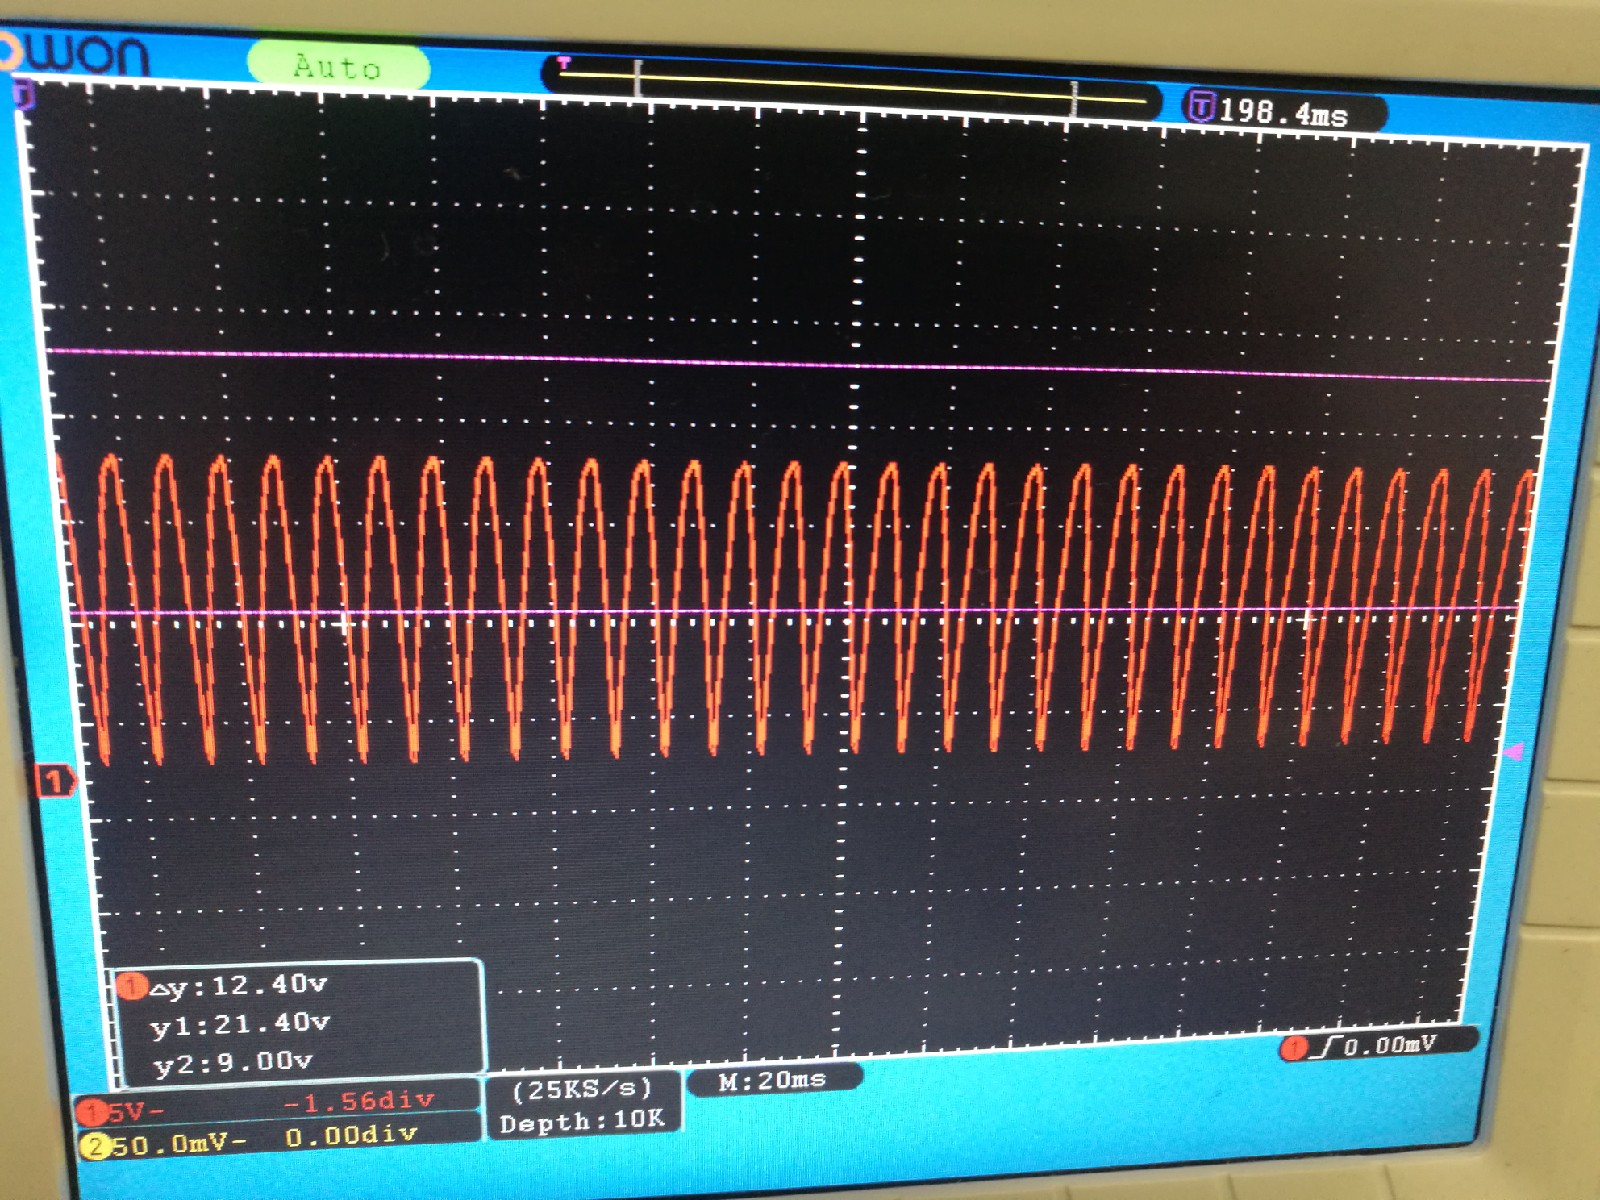
\includegraphics[width=1\linewidth]{5.jpg}} a) \\
	\end{minipage}
	\hfill
	\begin{minipage}[h]{0.47\linewidth}
		\center{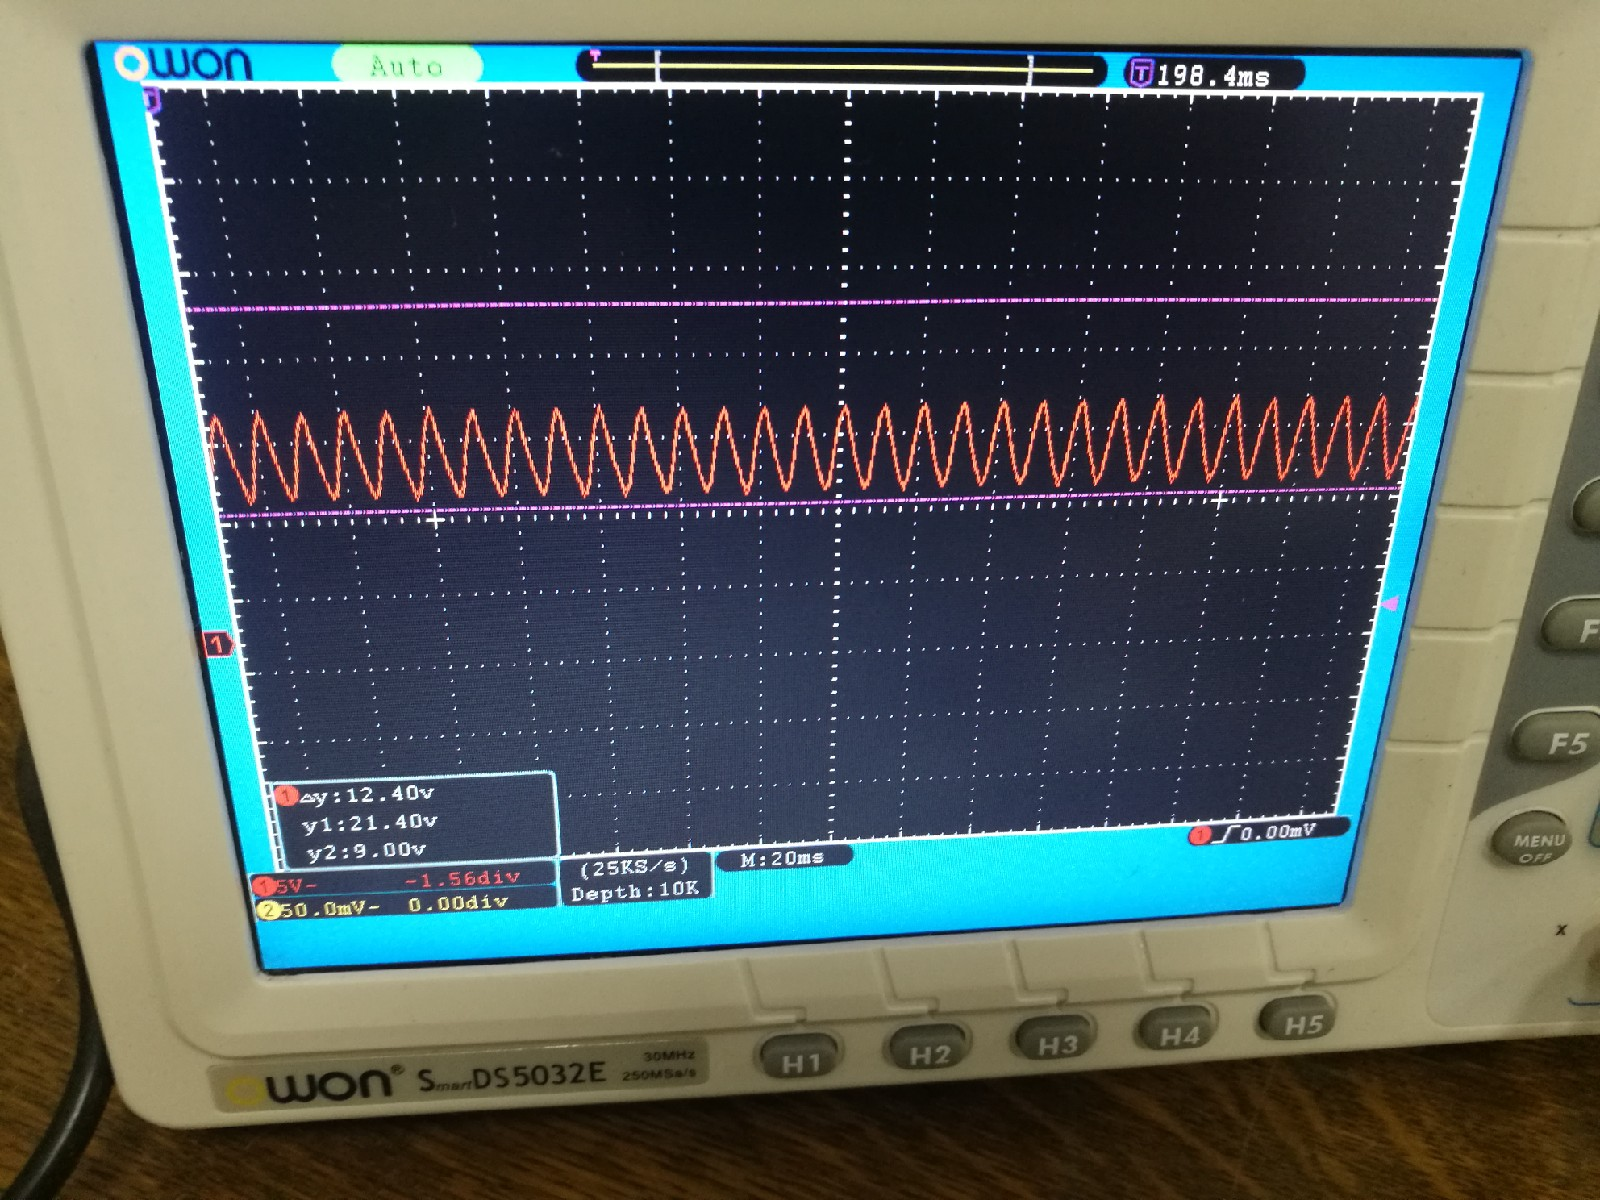
\includegraphics[width=1\linewidth]{6.jpg}} \\b)
	\end{minipage}
	\vfill
	\begin{minipage}[h]{0.47\linewidth}
		\center{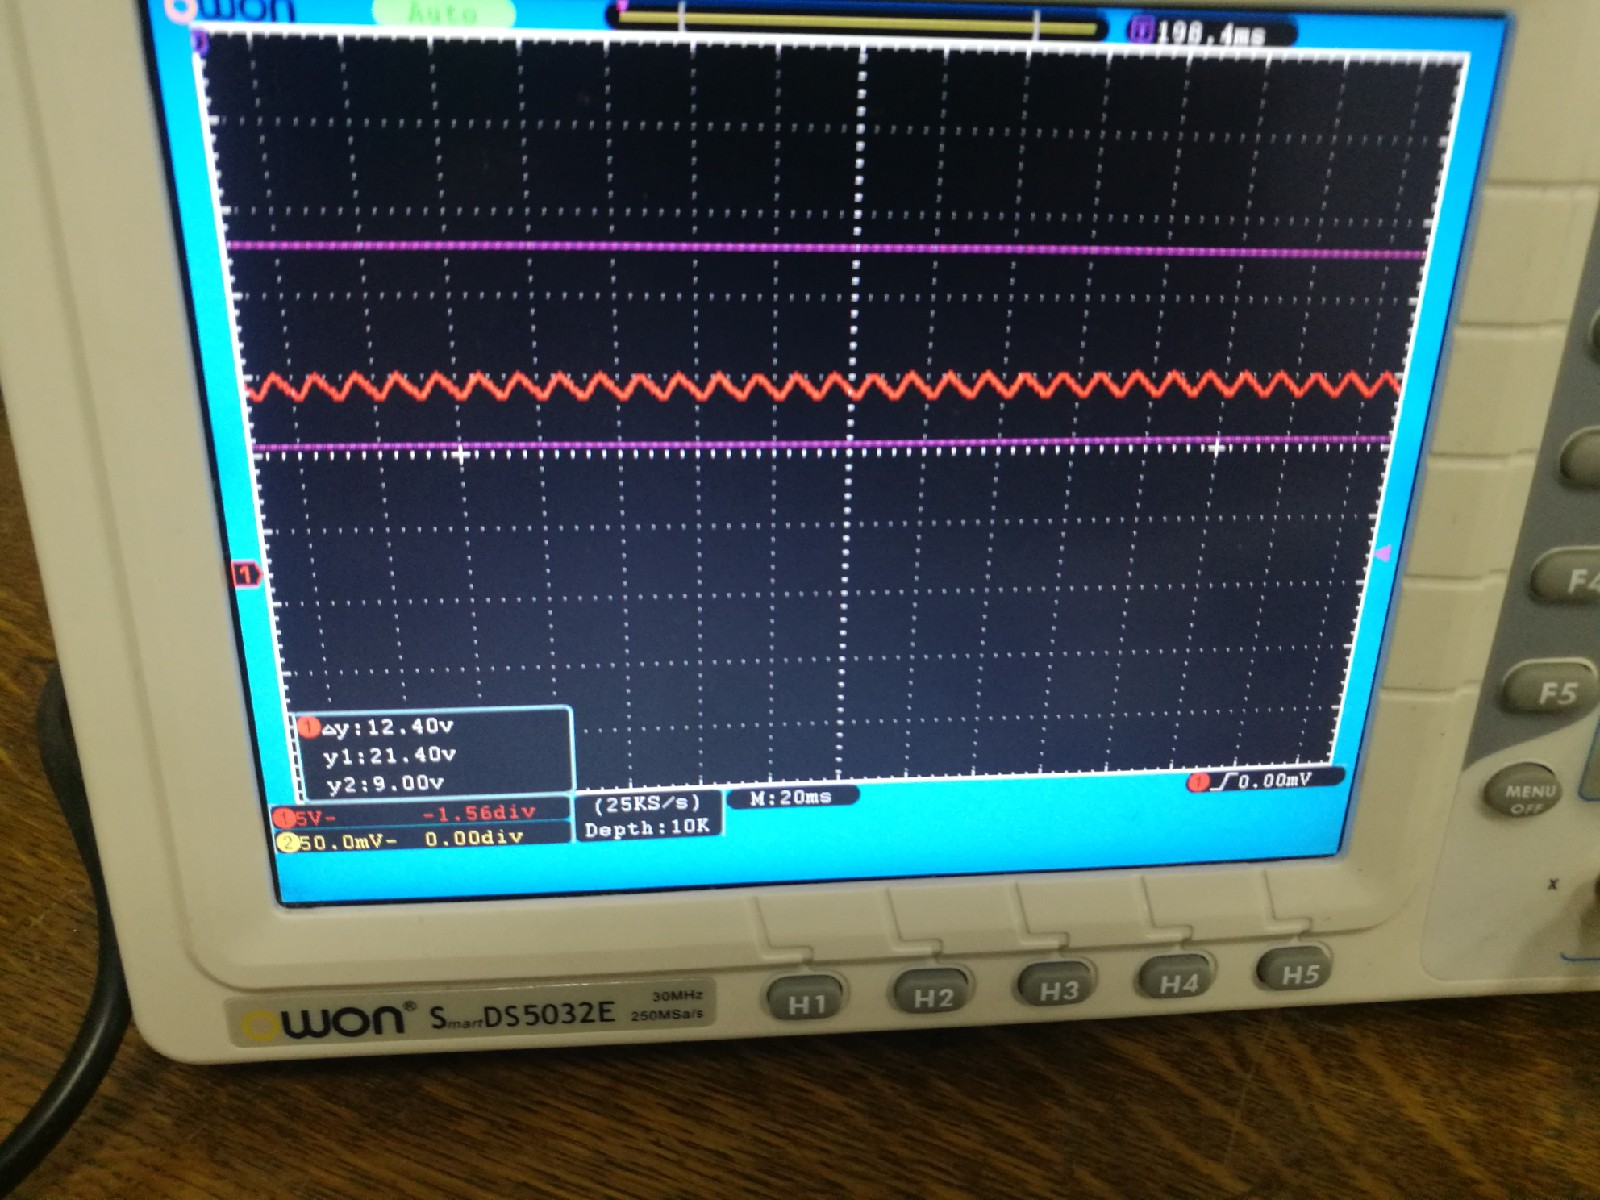
\includegraphics[width=1\linewidth]{7.jpg}} c) \\
	\end{minipage}
	\hfill
	\begin{minipage}[h]{0.47\linewidth}
		\center{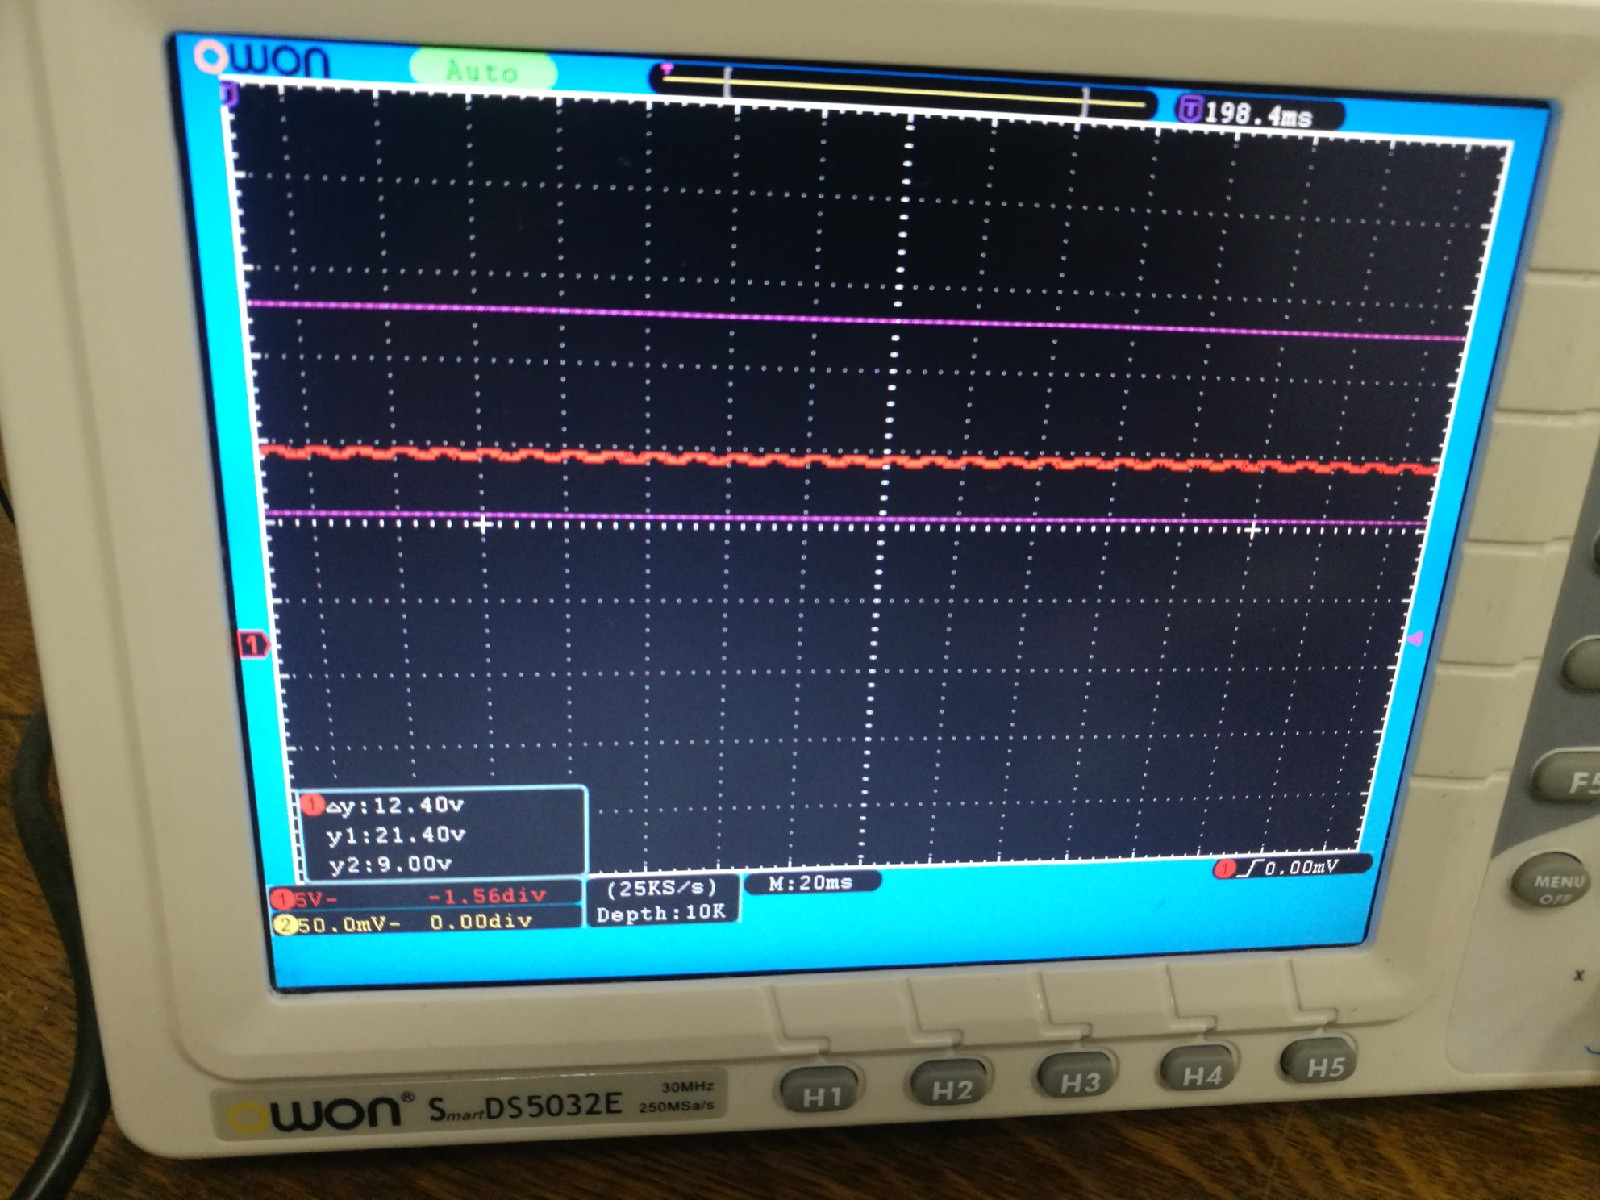
\includegraphics[width=1\linewidth]{8.jpg}} d) \\
	\end{minipage}
	\caption{Осциллограммы напряжения на выходе двухполупериодный мостикового выпрямителя со сглаживающими емкостями a)$C = 0$; b)$C_1$; c)$C_2 > C_1$; d)$C_3 > C_2$.}
	\label{ris:image6}
\end{figure}

\end{document}
